% Options for packages loaded elsewhere
\PassOptionsToPackage{unicode}{hyperref}
\PassOptionsToPackage{hyphens}{url}
\documentclass[
]{article}
\usepackage{xcolor}
\usepackage[margin=1in]{geometry}
\usepackage{amsmath,amssymb}
\setcounter{secnumdepth}{5}
\usepackage{iftex}
\ifPDFTeX
  \usepackage[T1]{fontenc}
  \usepackage[utf8]{inputenc}
  \usepackage{textcomp} % provide euro and other symbols
\else % if luatex or xetex
  \usepackage{unicode-math} % this also loads fontspec
  \defaultfontfeatures{Scale=MatchLowercase}
  \defaultfontfeatures[\rmfamily]{Ligatures=TeX,Scale=1}
\fi
\usepackage{lmodern}
\ifPDFTeX\else
  % xetex/luatex font selection
\fi
% Use upquote if available, for straight quotes in verbatim environments
\IfFileExists{upquote.sty}{\usepackage{upquote}}{}
\IfFileExists{microtype.sty}{% use microtype if available
  \usepackage[]{microtype}
  \UseMicrotypeSet[protrusion]{basicmath} % disable protrusion for tt fonts
}{}
\makeatletter
\@ifundefined{KOMAClassName}{% if non-KOMA class
  \IfFileExists{parskip.sty}{%
    \usepackage{parskip}
  }{% else
    \setlength{\parindent}{0pt}
    \setlength{\parskip}{6pt plus 2pt minus 1pt}}
}{% if KOMA class
  \KOMAoptions{parskip=half}}
\makeatother
\usepackage{longtable,booktabs,array}
\newcounter{none} % for unnumbered tables
\usepackage{calc} % for calculating minipage widths
% Correct order of tables after \paragraph or \subparagraph
\usepackage{etoolbox}
\makeatletter
\patchcmd\longtable{\par}{\if@noskipsec\mbox{}\fi\par}{}{}
\makeatother
% Allow footnotes in longtable head/foot
\IfFileExists{footnotehyper.sty}{\usepackage{footnotehyper}}{\usepackage{footnote}}
\makesavenoteenv{longtable}
\usepackage{graphicx}
\makeatletter
\newsavebox\pandoc@box
\newcommand*\pandocbounded[1]{% scales image to fit in text height/width
  \sbox\pandoc@box{#1}%
  \Gscale@div\@tempa{\textheight}{\dimexpr\ht\pandoc@box+\dp\pandoc@box\relax}%
  \Gscale@div\@tempb{\linewidth}{\wd\pandoc@box}%
  \ifdim\@tempb\p@<\@tempa\p@\let\@tempa\@tempb\fi% select the smaller of both
  \ifdim\@tempa\p@<\p@\scalebox{\@tempa}{\usebox\pandoc@box}%
  \else\usebox{\pandoc@box}%
  \fi%
}
% Set default figure placement to htbp
\def\fps@figure{htbp}
\makeatother
\setlength{\emergencystretch}{3em} % prevent overfull lines
\providecommand{\tightlist}{%
  \setlength{\itemsep}{0pt}\setlength{\parskip}{0pt}}
\usepackage[]{natbib}
\bibliographystyle{plainnat}
\usepackage{booktabs}
\usepackage{longtable}
\usepackage{array}
\usepackage{multirow}
\usepackage{wrapfig}
\usepackage{float}
\usepackage{colortbl}
\usepackage{pdflscape}
\usepackage{tabu}
\usepackage{threeparttable}
\usepackage{threeparttablex}
\usepackage[normalem]{ulem}
\usepackage{makecell}
\usepackage{xcolor}
\usepackage{bookmark}
\IfFileExists{xurl.sty}{\usepackage{xurl}}{} % add URL line breaks if available
\urlstyle{same}
\hypersetup{
  pdftitle={Social learning by type-token frequency - analysis},
  hidelinks,
  pdfcreator={LaTeX via pandoc}}

\title{Social learning by type-token frequency - analysis}
\author{Ansgar D. Endress\\
City, University of London}
\date{}

\begin{document}
\maketitle
\begin{abstract}
Abstract (to be written). Argument structure - See below. Analysis structure - 1. Descriptives of difference scores and tests against zero. 2. GLMMs, with reference to ANOVA. Discuss quorum sensing \citep{Sumpter2009} Discuss moral repetition effect, and tolerance principle and submit to psych sci. In intro. Different formal perspectives suggest that mere frequency should not be relevant, From a learning perspective, {[}Explanation of tolerance principle; argue later that threshold is 8/ln(8) = 3.8, but that we did not vary this experimentally as it's too long; general explanation of tolerance principle- When having a productive rule is faster than listing all items as exception{]}. From a representational perspective, dispositions. intrinsic properties of banana; bayesian argument. From a social perspective, majority. Whatever the moral frequency guy argues.
\end{abstract}

\section{Methods (continued)}\label{methods-continued}

\subsection{Exclusions}\label{exclusions}

I excluded 0 participants because they failed the attention test.

\subsection{SD3 REMOVE THIS IN PAPER}\label{sd3-remove-this-in-paper}

We next analyze the SD3 and combine the results with the data frame for the main experiment.

\begin{table}
\centering
\caption{\label{tab:analyze-sd3-add-median-split}Number of participants in each group of the SD3 scales. Note that this applies to city students only}
\centering
\begin{tabular}[t]{lrrrrrr}
\toprule
\multicolumn{1}{c}{\textbf{ }} & \multicolumn{3}{c}{\textbf{N}} & \multicolumn{3}{c}{\textbf{Percentage}} \\
\cmidrule(l{3pt}r{3pt}){2-4} \cmidrule(l{3pt}r{3pt}){5-7}
scale & high & low & NA\_ & high & low & NA\_\\
\midrule
Machiavellianism & 23 & 24 & 5 & 0.442 & 0.462 & 0.096\\
Narcissism & 26 & 26 & 0 & 0.500 & 0.500 & 0.000\\
Psychopathy & 25 & 24 & 3 & 0.481 & 0.462 & 0.058\\
\bottomrule
\end{tabular}
\end{table}

\clearpage

\subsection{Analysis strategy}\label{analysis-strategy}

I analyzed the data in three stages. First, I present descriptives of the raw ratings to serve as task validations, as good actions should be rated as morally better than bad actions. However, I had no other predictions for the raw levels of acceptability.

Second, for each domain (first-party acceptability, third-party acceptability, prevalence), I calculated two types of difference scores. Following \citep{Rosenthal1999}, I used focused difference scores (rather than models with effects for which I had no predictions) to target the contrasts of interest, also ensuring consistency between visualizations and statistical tests. The first type of difference score assesses the effect of type and token frequency compared to single occurrence events, namely \(\frac{\text{High Type-Frequency} - \text{Single Occurrence}}{\text{High Type-Frequency} + \text{Single Occurrence}}\) and \(\frac{\text{Low Type-Frequency} - \text{Single Occurrence}}{\text{Low Type-Frequency} + \text{Single Occurrence}}\). I compared these difference scores to the chance level of zero using Wilcoxon tests.

The second type of difference score compared the effects of type and token frequency with each other, specifically \(\frac{\text{High Type-Frequency} - \text{Low Type-Frequency}}{\text{High Type-Frequency} + \text{Low Type-Frequency}}\). Again, I compared these difference scores to the chance level of zero. For both types of difference scores, I also asked whether they would be affected by the valence. P-values were corrected using the Holm-Bonferroni method.

Finally, I used a series of Cumulative Linear Mixed Model (CLMM) with a logit link function to confirm these results \citep{Buerkner2019, Liddell2018}, using the ordinal \(R\) package \citep{ordinal}. CLMMs assume that participant responses reflect an underlying latent variable. The model estimates multiple thresholds corresponding to different response categories, with a response given when the latent variable exceeds the threshold for that category. In addition to the thresholds, they also estimate linear predictors influencing the latent variable.

NOTE TO SELF: THERE ARE ALSO SEQUENTIAL MODELS, SEE \citep{Buerkner2019}.

Problems with treating ordinal responses \citep{Liddell2018}

\url{https://pmc.ncbi.nlm.nih.gov/articles/PMC10439063/}
\citep{Taylor2023} this is about norms

\subsection{Participants}\label{participants}

\begin{table}
\centering
\caption{\label{tab:print-demographics}Demographics of the final sample}
\centering
\begin{tabular}[t]{l|r|r|r|r|r|l}
\hline
\multicolumn{5}{c|}{\textbf{ }} & \multicolumn{2}{c}{\textbf{Age}} \\
\cline{6-7}
population & N & Females & Males & Other & Age.m & Age.range\\
\hline
students & 52 & 48 & 3 & 1 & 18.5 & 18-22\\
\hline
testable & 119 & 59 & 59 & 1 & 32.7 & 18-61\\
\hline
\end{tabular}
\end{table}

\clearpage

\section{Results}\label{results}

\subsection{Raw ratings}\label{raw-ratings}

\begin{figure}

{\centering 
\includegraphics[width=0.8\linewidth]{social_learning_type_token_sequential_results_files/figure-latex/plot-ratings-raw-1} 

}

\caption{Ratings for (a) testable participants and (b) students. The dots, error bars and violin represent the sample average, 95\% bootstrap confidence intervals and the distribution of the individual responses, respectively. Open circles represent individual participants.}\label{fig:plot-ratings-raw}
\end{figure}

The raw ratings are shown in Figure \ref{fig:plot-ratings-raw} and Table \ref{tab:print-descriptives-ratings-raw2}. As shown in Table \ref{tab:clmm-raw-effects-of-valency2}, a CLMM with a logit link function, including the fixed predictors Valence and Frequency Condition, their interaction, and a random slope for participants---showed that, for both acceptability questions and both samples, good deeds were judged more positively than neutral ones, and neutral ones more positively than bad ones. The valence manipulation was thus successful.

\clearpage

\subsection{Comparisons of the high and low type-frequency conditions against the single occurrence condition}\label{comparisons-of-the-high-and-low-type-frequency-conditions-against-the-single-occurrence-condition}

I next turned to the question of whether type-frequency or token-frequency would affect acceptability and prevalence judgments, using the difference scores that compared each frequency condition to the single-occurrence condition.

\subsubsection{Difference scores}\label{difference-scores}

\begin{figure}

{\centering 
\includegraphics[width=0.8\linewidth]{social_learning_type_token_sequential_results_files/figure-latex/plot-difference-vs-single-raw-1} 

}

\caption{Difference scores against the single occurrence condition ($\frac{\text{High Type-Frequency} - \text{Single Occurrence}}{\text{High Type-Frequency} + \text{Single Occurrence}}$ and $\frac{\text{Low Type-Frequency} - \text{Single Occurrence}}{\text{Low Type-Frequency} + \text{Single Occurrence}}$). The dot, error bars and violin represent the sample average, 95\% bootstrap confidence intervals and the distribution of the individual responses, respectively. Open circles represent individual participants. Significance codes: *** $p \leq .001$, ** $p \leq .01$, * $p \leq .05$, . $p \leq .10$, ns = not significant.}\label{fig:plot-difference-vs-single-raw}
\end{figure}

The results are shown in Figures \ref{fig:plot-difference-vs-single-raw} and Table \ref{tab:difference-vs-single-raw-print2}. For first-party acceptability, ratings in the high type frequency condition differed reliably from those in the single occurrence condition, mainly for good and neutral actions. For bad actions, while the uncorrected effect was significant, it became marginal after correction in the testable sample, and non-significant in the student sample. In contrast, ratings in the low type frequency condition did not significantly differ from those in the single occurrence condition. First-party acceptability thus seems primarily driven by type rather than token frequency.

To provide evidence for the null hypothesis, I fit two linear models to the first-party acceptability difference scores: one representing the null hypothesis (with the mean fixed at 0) and one representing the alternative hypothesis (with the mean estimated from the data). I then calculated the likelihood of the data under each model, applied corrections for the numbers of parameters using the Bayesian Information Criterion (BIC) and the Akaike Information Criterion (AIC), and computed the likelihood ratio, with values greater than one indicating support for the null hypothesis. As shown in Table \ref{tab:difference-vs-single-raw-print2}, the first-party acceptability difference scores comparing the low type-frequency condition to the single-occurrence condition generally provided weak to moderate evidence in favor of the null hypothesis, suggesting again that first-party acceptability is primarily driven by type frequency rather than token frequency.

For both third-party acceptability and prevalence, ratings in both the high and low type frequency conditions differed from the single occurrence condition across all valence conditions, though the difference scores were roughly twice as large for the high type frequency condition compared to the low type frequency condition. Both type and token frequency thus affect these ratings, though I will demonstrate below that the effect of type frequency is substantially larger.

\clearpage

\subsubsection{Confirmation with ordinal model}\label{confirmation-with-ordinal-model}

I confirmed these results with a series of CLMMs. For each domain (acceptability and prevalence), I included the fixed factor predictors Frequency Condition (High Type-Frequency vs.~Single Occurrence and Low Type-Frequency vs.~Single Occurrence) and Valence (with the reference level set to neutral), as well as a random slope for participants.

\begin{longtable}[t]{lrrrrrrl}
\caption{\label{tab:clmm-vs-single-occurrence-print}Results from a set of cumulative link mixed models, fitted separately for each sample (testable and students), domain (First-Party Acceptability, Third-Party Acceptability, and Prevalence), and frequency contrast (High Type-Frequency vs. Single Occurrence and Low Type-Frequency vs. Single Occurrence), with fixed factor predictors Frequency Condition and Valence, their interaction, and a random slope for participants. For the Low Type-Frequency vs. Single Occurrence contrast in Third-Party Acceptability, the Valence $\times$ Frequency Condition interaction was omitted (additive model used) due to complete separation caused by zero observations at the lowest rating for good actions in the testable sample. Significance codes: *** $p \leq .001$, ** $p \leq .01$, * $p \leq .05$, . $p \leq .10$, ns = not significant.}\\
\toprule
Parameter & Coefficient & $\mathit{SE}$ & $CI_{\text{low}}$ & $CI_{\text{high}}$ & z & $p$ &  \\
\midrule
\endfirsthead
\caption[]{\label{tab:clmm-vs-single-occurrence-print}Results from a set of cumulative link mixed models, fitted separately for each sample (testable and students), domain (First-Party Acceptability, Third-Party Acceptability, and Prevalence), and frequency contrast (High Type-Frequency vs. Single Occurrence and Low Type-Frequency vs. Single Occurrence), with fixed factor predictors Frequency Condition and Valence, their interaction, and a random slope for participants. For the Low Type-Frequency vs. Single Occurrence contrast in Third-Party Acceptability, the Valence $\times$ Frequency Condition interaction was omitted (additive model used) due to complete separation caused by zero observations at the lowest rating for good actions in the testable sample. Significance codes: *** $p \leq .001$, ** $p \leq .01$, * $p \leq .05$, . $p \leq .10$, ns = not significant. \textit{(continued)}}\\
\toprule
Parameter & Coefficient & $\mathit{SE}$ & $CI_{\text{low}}$ & $CI_{\text{high}}$ & z & $p$ &  \\
\midrule
\endhead

\endfoot
\bottomrule
\endlastfoot
\addlinespace[0.3em]
\multicolumn{8}{l}{\textbf{First Party Acceptability - High Type-Frequency (vs. Single Occurrence) - Students}}\\
\hspace{1em}Valence:bad & -2.024 & 0.107 & -2.234 & -1.813 & -18.856 & 0.000 & ***\\
\hspace{1em}Valence:good & 2.891 & 0.109 & 2.678 & 3.105 & 26.524 & 0.000 & ***\\
Freq.
Cond:high
\hspace{1em}Type-Freq. & 0.757 & 0.086 & 0.588 & 0.926 & 8.772 & 0.000 & ***\\
Valence:bad$\times$Freq.
Cond:high
\hspace{1em}Type-Freq. & -0.602 & 0.102 & -0.803 & -0.402 & -5.893 & 0.000 & ***\\
Valence:good$\times$Freq.
Cond:high
\hspace{1em}Type-Freq. & -0.516 & 0.148 & -0.806 & -0.226 & -3.484 & 0.000 & ***\\
\addlinespace[0.3em]
\multicolumn{8}{l}{\textbf{First Party Acceptability - High Type-Frequency (vs. Single Occurrence) - Testable}}\\
\hspace{1em}Valence:bad & -3.946 & 0.307 & -4.548 & -3.344 & -12.854 & 0.000 & ***\\
\hspace{1em}Valence:good & 2.147 & 0.315 & 1.529 & 2.766 & 6.807 & 0.000 & ***\\
Freq.
Cond:high
\hspace{1em}Type-Freq. & 0.471 & 0.130 & 0.216 & 0.726 & 3.626 & 0.000 & ***\\
Valence:bad$\times$Freq.
Cond:high
\hspace{1em}Type-Freq. & -0.241 & 0.205 & -0.644 & 0.161 & -1.176 & 0.240 & ns\\
Valence:good$\times$Freq.
Cond:high
\hspace{1em}Type-Freq. & 0.136 & 0.215 & -0.286 & 0.559 & 0.633 & 0.526 & ns\\
\addlinespace[0.3em]
\multicolumn{8}{l}{\textbf{First Party Acceptability - Low Type-Frequency (vs. Single Occurrence) - Students}}\\
\hspace{1em}Valence:bad & -2.094 & 0.435 & -2.946 & -1.242 & -4.818 & 0.000 & ***\\
\hspace{1em}Valence:good & 2.940 & 0.443 & 2.072 & 3.807 & 6.642 & 0.000 & ***\\
Freq.
Cond:low
\hspace{1em}Type-Freq. & 0.303 & 0.193 & -0.074 & 0.681 & 1.575 & 0.115 & ns\\
Valence:bad$\times$Freq.
Cond:low
\hspace{1em}Type-Freq. & -0.267 & 0.277 & -0.810 & 0.276 & -0.962 & 0.336 & ns\\
Valence:good$\times$Freq.
Cond:low
\hspace{1em}Type-Freq. & -0.149 & 0.300 & -0.737 & 0.439 & -0.497 & 0.619 & ns\\
\addlinespace[0.3em]
\multicolumn{8}{l}{\textbf{First Party Acceptability - Low Type-Frequency (vs. Single Occurrence) - Testable}}\\
\hspace{1em}Valence:bad & -4.025 & 0.335 & -4.681 & -3.369 & -12.022 & 0.000 & ***\\
\hspace{1em}Valence:good & 2.189 & 0.331 & 1.541 & 2.837 & 6.623 & 0.000 & ***\\
Freq.
Cond:low
\hspace{1em}Type-Freq. & 0.187 & 0.129 & -0.065 & 0.440 & 1.453 & 0.146 & ns\\
Valence:bad$\times$Freq.
Cond:low
\hspace{1em}Type-Freq. & -0.082 & 0.208 & -0.490 & 0.325 & -0.397 & 0.691 & ns\\
Valence:good$\times$Freq.
Cond:low
\hspace{1em}Type-Freq. & 0.002 & 0.207 & -0.405 & 0.408 & 0.008 & 0.994 & ns\\
\addlinespace[0.3em]
\multicolumn{8}{l}{\textbf{Third Party Acceptability - High Type-Frequency (vs. Single Occurrence) - Students}}\\
\hspace{1em}Valence:bad & -1.609 & 0.398 & -2.389 & -0.828 & -4.040 & 0.000 & ***\\
\hspace{1em}Valence:good & 1.745 & 0.393 & 0.974 & 2.516 & 4.435 & 0.000 & ***\\
Freq.
Cond:high
\hspace{1em}Type-Freq. & 3.019 & 0.221 & 2.586 & 3.452 & 13.669 & 0.000 & ***\\
Valence:bad$\times$Freq.
Cond:high
\hspace{1em}Type-Freq. & -0.456 & 0.282 & -1.009 & 0.097 & -1.616 & 0.106 & ns\\
Valence:good$\times$Freq.
Cond:high
\hspace{1em}Type-Freq. & -0.225 & 0.310 & -0.833 & 0.382 & -0.727 & 0.468 & ns\\
\addlinespace[0.3em]
\multicolumn{8}{l}{\textbf{Third Party Acceptability - High Type-Frequency (vs. Single Occurrence) - Testable}}\\
\hspace{1em}Valence:bad & -2.230 & 0.326 & -2.869 & -1.591 & -6.840 & 0.000 & ***\\
\hspace{1em}Valence:good & 1.502 & 0.330 & 0.855 & 2.148 & 4.552 & 0.000 & ***\\
Freq.
Cond:high
\hspace{1em}Type-Freq. & 2.438 & 0.150 & 2.144 & 2.732 & 16.255 & 0.000 & ***\\
Valence:bad$\times$Freq.
Cond:high
\hspace{1em}Type-Freq. & 0.282 & 0.194 & -0.098 & 0.661 & 1.453 & 0.146 & ns\\
Valence:good$\times$Freq.
Cond:high
\hspace{1em}Type-Freq. & -0.182 & 0.227 & -0.627 & 0.263 & -0.800 & 0.424 & ns\\
\addlinespace[0.3em]
\multicolumn{8}{l}{\textbf{Third Party Acceptability - Low Type-Frequency (vs. Single Occurrence) - Students}}\\
\hspace{1em}Valence:bad & -2.238 & 0.516 & -3.249 & -1.226 & -4.336 & 0.000 & ***\\
\hspace{1em}Valence:good & 2.100 & 0.511 & 1.097 & 3.102 & 4.106 & 0.000 & ***\\
Freq.
Cond:low
\hspace{1em}Type-Freq. & 1.090 & 0.119 & 0.857 & 1.323 & 9.166 & 0.000 & ***\\
\addlinespace[0.3em]
\multicolumn{8}{l}{\textbf{Third Party Acceptability - Low Type-Frequency (vs. Single Occurrence) - Testable}}\\
\hspace{1em}Valence:bad & -2.070 & 0.287 & -2.633 & -1.507 & -7.210 & 0.000 & ***\\
\hspace{1em}Valence:good & 1.679 & 0.382 & 0.931 & 2.427 & 4.397 & 0.000 & ***\\
Freq.
Cond:low
\hspace{1em}Type-Freq. & 1.209 & 0.130 & 0.955 & 1.462 & 9.329 & 0.000 & ***\\
\addlinespace[0.3em]
\multicolumn{8}{l}{\textbf{Prevalence - High Type-Frequency (vs. Single Occurrence) - Students}}\\
\hspace{1em}Valence:bad & 0.493 & 0.354 & -0.201 & 1.187 & 1.392 & 0.164 & ns\\
\hspace{1em}Valence:good & 2.125 & 0.356 & 1.427 & 2.823 & 5.969 & 0.000 & ***\\
Freq.
Cond:high
\hspace{1em}Type-Freq. & 4.409 & 0.248 & 3.922 & 4.896 & 17.750 & 0.000 & ***\\
Valence:bad$\times$Freq.
Cond:high
\hspace{1em}Type-Freq. & -0.607 & 0.289 & -1.173 & -0.040 & -2.100 & 0.036 & *\\
Valence:good$\times$Freq.
Cond:high
\hspace{1em}Type-Freq. & -1.085 & 0.310 & -1.694 & -0.477 & -3.497 & 0.000 & ***\\
\addlinespace[0.3em]
\multicolumn{8}{l}{\textbf{Prevalence - High Type-Frequency (vs. Single Occurrence) - Testable}}\\
\hspace{1em}Valence:bad & -0.156 & 0.326 & -0.795 & 0.484 & -0.477 & 0.633 & ns\\
\hspace{1em}Valence:good & 1.790 & 0.333 & 1.137 & 2.443 & 5.371 & 0.000 & ***\\
Freq.
Cond:high
\hspace{1em}Type-Freq. & 4.255 & 0.174 & 3.914 & 4.596 & 24.455 & 0.000 & ***\\
Valence:bad$\times$Freq.
Cond:high
\hspace{1em}Type-Freq. & -0.750 & 0.206 & -1.153 & -0.346 & -3.643 & 0.000 & ***\\
Valence:good$\times$Freq.
Cond:high
\hspace{1em}Type-Freq. & -1.111 & 0.229 & -1.561 & -0.662 & -4.846 & 0.000 & ***\\
\addlinespace[0.3em]
\multicolumn{8}{l}{\textbf{Prevalence - Low Type-Frequency (vs. Single Occurrence) - Students}}\\
\hspace{1em}Valence:bad & 0.541 & 0.522 & -0.482 & 1.565 & 1.037 & 0.300 & ns\\
\hspace{1em}Valence:good & 2.519 & 0.521 & 1.499 & 3.540 & 4.839 & 0.000 & ***\\
Freq.
Cond:low
\hspace{1em}Type-Freq. & 1.922 & 0.219 & 1.493 & 2.350 & 8.783 & 0.000 & ***\\
Valence:bad$\times$Freq.
Cond:low
\hspace{1em}Type-Freq. & 0.068 & 0.287 & -0.495 & 0.631 & 0.236 & 0.813 & ns\\
Valence:good$\times$Freq.
Cond:low
\hspace{1em}Type-Freq. & -0.094 & 0.294 & -0.670 & 0.482 & -0.321 & 0.748 & ns\\
\addlinespace[0.3em]
\multicolumn{8}{l}{\textbf{Prevalence - Low Type-Frequency (vs. Single Occurrence) - Testable}}\\
\hspace{1em}Valence:bad & -0.212 & 0.401 & -0.998 & 0.573 & -0.530 & 0.596 & ns\\
\hspace{1em}Valence:good & 2.043 & 0.409 & 1.241 & 2.845 & 4.993 & 0.000 & ***\\
Freq.
Cond:low
\hspace{1em}Type-Freq. & 1.759 & 0.137 & 1.490 & 2.028 & 12.810 & 0.000 & ***\\
Valence:bad$\times$Freq.
Cond:low
\hspace{1em}Type-Freq. & 0.365 & 0.185 & 0.002 & 0.728 & 1.968 & 0.049 & *\\
Valence:good$\times$Freq.
Cond:low
\hspace{1em}Type-Freq. & -0.253 & 0.191 & -0.627 & 0.121 & -1.324 & 0.186 & ns\\*
\end{longtable}

The results are shown in Table \ref{tab:clmm-vs-single-occurrence-print}. For first-party acceptability, ratings differed significantly from the single-occurrence condition only in the high type-frequency condition, confirming that first-party acceptability is primarily driven by type frequency. (In the student sample, some additional interactions emerged, but these could not be replicated in the testable sample.)

For third-party acceptability and prevalence, both the high and low type-frequency conditions differed from the single-occurrence condition (except for the low type-frequency condition in third-party acceptability ratings within the student sample). However, the parameter estimates were approximately two to three times greater for the high type-frequency condition than for the low type-frequency condition.

For prevalence, the effect of high type-frequency was reduced for good and bad actions relative to neutral actions, while the effect of token frequency was slightly stronger for bad actions in the testable sample.

\subsection{Comparisons of the high and low type-frequency conditions}\label{comparisons-of-the-high-and-low-type-frequency-conditions}

I now turn to the question of whether type and token frequency affect ratings differentially. I first address this question using difference scores, and then confirm these results using an CLMM.

\subsubsection{Difference scores}\label{difference-scores-1}

\begin{figure}

{\centering 
\includegraphics[width=0.8\linewidth]{social_learning_type_token_sequential_results_files/figure-latex/plot-difference-high-vs-low-type-frequency-raw-1} 

}

\caption{Difference scores comparing the High and Low Type-Frequency Conditions ($\frac{\text{High Type-Frequency} - \text{Low Type-Frequency}}{\text{High Type-Frequency} + \text{Low Type-Frequency}}$). The dots, error bars and violin represent the sample average, 95\% bootstrap confidence intervals and the distribution of the individual responses, respectively. Open circles represent individual participants. Significance codes: *** $p \leq .001$, ** $p \leq .01$, * $p \leq .05$, . $p \leq .10$, ns = not significant.}\label{fig:plot-difference-high-vs-low-type-frequency-raw}
\end{figure}

The results are shown in Figure \ref{fig:plot-difference-high-vs-low-type-frequency-raw} and Table \ref{tab:difference-high-vs-low-type-frequency-print1}. For first-party acceptability, the difference scores were significantly greater than zero for good and neutral actions in the testable sample, and for neutral actions only in the student sample. First-party acceptability ratings thus increase when the type frequency of an action is increased, even when the frequency of occurrence is held constant.

For third-party acceptability and prevalence, the difference scores were significantly greater than zero for all valence conditions and samples, showing again that type-frequency has an effect over and above frequency of occurrence.

\clearpage

\subsubsection{Confirmation with ordinal model}\label{confirmation-with-ordinal-model-1}

I confirmed these results with a series of CLMMs. For each domain, I fitted a model including the fixed factor predictors Frequency Condition (High Type-Frequency vs.~Low Type-Frequency) and Valence, with the reference level set to neutral.

\begin{longtable}[t]{lrrrrrrl}
\caption{\label{tab:clmm-high-vs-low-type-frequency-print}Results from a set of cumulative link mixed models, contrasting the High Type-Frequency condition with the Low Type-Frequency condition. Models were fitted separately for each sample (online or student) and domain (Prevalence, First-Party Acceptability, and Third-Party Acceptability), with fixed factor predictors Valence, Frequency Condition, and their interaction, as well as a random slope for participants. Significance codes: *** $p \leq .001$, ** $p \leq .01$, * $p \leq .05$, . $p \leq .10$, ns = not significant.}\\
\toprule
Parameter & Coefficient & $\mathit{SE}$ & $CI_{\text{low}}$ & $CI_{\text{high}}$ & z & $p$ &  \\
\midrule
\endfirsthead
\caption[]{\label{tab:clmm-high-vs-low-type-frequency-print}Results from a set of cumulative link mixed models, contrasting the High Type-Frequency condition with the Low Type-Frequency condition. Models were fitted separately for each sample (online or student) and domain (Prevalence, First-Party Acceptability, and Third-Party Acceptability), with fixed factor predictors Valence, Frequency Condition, and their interaction, as well as a random slope for participants. Significance codes: *** $p \leq .001$, ** $p \leq .01$, * $p \leq .05$, . $p \leq .10$, ns = not significant. \textit{(continued)}}\\
\toprule
Parameter & Coefficient & $\mathit{SE}$ & $CI_{\text{low}}$ & $CI_{\text{high}}$ & z & $p$ &  \\
\midrule
\endhead

\endfoot
\bottomrule
\endlastfoot
\addlinespace[0.3em]
\multicolumn{8}{l}{\textbf{First Party Acceptability - Students}}\\
\hspace{1em}Valence:bad & -2.348 & 0.424 & -3.179 & -1.518 & -5.542 & 0.000 & ***\\
\hspace{1em}Valence:good & 2.798 & 0.432 & 1.951 & 3.645 & 6.476 & 0.000 & ***\\
Freq.
Cond:high
\hspace{1em}Type-Freq. & 0.485 & 0.192 & 0.109 & 0.862 & 2.525 & 0.012 & *\\
Valence:bad$\times$Freq.
Cond:high
\hspace{1em}Type-Freq. & -0.364 & 0.277 & -0.906 & 0.178 & -1.315 & 0.188 & ns\\
Valence:good$\times$Freq.
Cond:high
\hspace{1em}Type-Freq. & -0.397 & 0.304 & -0.993 & 0.199 & -1.306 & 0.192 & ns\\
\addlinespace[0.3em]
\multicolumn{8}{l}{\textbf{First Party Acceptability - Testable}}\\
\hspace{1em}Valence:bad & -4.139 & 0.327 & -4.781 & -3.498 & -12.654 & 0.000 & ***\\
\hspace{1em}Valence:good & 2.172 & 0.330 & 1.525 & 2.819 & 6.576 & 0.000 & ***\\
Freq.
Cond:high
\hspace{1em}Type-Freq. & 0.272 & 0.131 & 0.016 & 0.528 & 2.079 & 0.038 & *\\
Valence:bad$\times$Freq.
Cond:high
\hspace{1em}Type-Freq. & -0.138 & 0.205 & -0.540 & 0.264 & -0.674 & 0.500 & ns\\
Valence:good$\times$Freq.
Cond:high
\hspace{1em}Type-Freq. & 0.156 & 0.220 & -0.276 & 0.588 & 0.709 & 0.479 & ns\\
\addlinespace[0.3em]
\multicolumn{8}{l}{\textbf{Third Party Acceptability - Students}}\\
\hspace{1em}Valence:bad & -2.010 & 0.416 & -2.824 & -1.195 & -4.836 & 0.000 & ***\\
\hspace{1em}Valence:good & 2.158 & 0.419 & 1.336 & 2.980 & 5.146 & 0.000 & ***\\
Freq.
Cond:high
\hspace{1em}Type-Freq. & 2.111 & 0.211 & 1.698 & 2.524 & 10.017 & 0.000 & ***\\
Valence:bad$\times$Freq.
Cond:high
\hspace{1em}Type-Freq. & -0.141 & 0.281 & -0.692 & 0.410 & -0.501 & 0.616 & ns\\
Valence:good$\times$Freq.
Cond:high
\hspace{1em}Type-Freq. & -0.549 & 0.316 & -1.169 & 0.071 & -1.736 & 0.083 & .\\
\addlinespace[0.3em]
\multicolumn{8}{l}{\textbf{Third Party Acceptability - Testable}}\\
\hspace{1em}Valence:bad & -1.598 & 0.424 & -2.428 & -0.768 & -3.772 & 0.000 & ***\\
\hspace{1em}Valence:good & 1.817 & 0.439 & 0.957 & 2.677 & 4.141 & 0.000 & ***\\
Freq.
Cond:high
\hspace{1em}Type-Freq. & 1.673 & 0.153 & 1.372 & 1.973 & 10.909 & 0.000 & ***\\
Valence:bad$\times$Freq.
Cond:high
\hspace{1em}Type-Freq. & -0.346 & 0.198 & -0.734 & 0.042 & -1.747 & 0.081 & .\\
Valence:good$\times$Freq.
Cond:high
\hspace{1em}Type-Freq. & -0.415 & 0.240 & -0.886 & 0.056 & -1.726 & 0.084 & .\\
\addlinespace[0.3em]
\multicolumn{8}{l}{\textbf{Prevalence - Students}}\\
\hspace{1em}Valence:bad & 0.699 & 0.440 & -0.164 & 1.562 & 1.587 & 0.113 & ns\\
\hspace{1em}Valence:good & 2.336 & 0.445 & 1.464 & 3.208 & 5.252 & 0.000 & ***\\
Freq.
Cond:high
\hspace{1em}Type-Freq. & 2.932 & 0.222 & 2.496 & 3.368 & 13.188 & 0.000 & ***\\
Valence:bad$\times$Freq.
Cond:high
\hspace{1em}Type-Freq. & -0.656 & 0.291 & -1.227 & -0.086 & -2.255 & 0.024 & *\\
Valence:good$\times$Freq.
Cond:high
\hspace{1em}Type-Freq. & -1.090 & 0.313 & -1.704 & -0.476 & -3.479 & 0.001 & ***\\
\addlinespace[0.3em]
\multicolumn{8}{l}{\textbf{Prevalence - Testable}}\\
\hspace{1em}Valence:bad & 0.261 & 0.448 & -0.617 & 1.140 & 0.583 & 0.560 & ns\\
\hspace{1em}Valence:good & 1.641 & 0.458 & 0.742 & 2.539 & 3.579 & 0.000 & ***\\
Freq.
Cond:high
\hspace{1em}Type-Freq. & 2.878 & 0.167 & 2.551 & 3.206 & 17.220 & 0.000 & ***\\
Valence:bad$\times$Freq.
Cond:high
\hspace{1em}Type-Freq. & -0.999 & 0.215 & -1.420 & -0.578 & -4.655 & 0.000 & ***\\
Valence:good$\times$Freq.
Cond:high
\hspace{1em}Type-Freq. & -1.066 & 0.233 & -1.522 & -0.610 & -4.583 & 0.000 & ***\\*
\end{longtable}

The results are shown in Table \ref{tab:clmm-high-vs-low-type-frequency-print}. In all domains and samples, ratings in the high type-frequency condition were higher than those in the low type-frequency condition.

We also observed main effects of valence, showing that good actions were rated higher than neutral ones, while neutral ones were rated higher than bad ones (except for prevalence ratings, where the latter two conditions did not differ).
These results thus mirror those of the difference scores above.''

\clearpage

\subsection{Alternative analyses}\label{alternative-analyses}

In SI \ref{app:alternative-analyses}, I report two alternative sets of analyses in addition to the difference score analyses and the CLMMs. First, I fit a series of generalized linear mixed models (GLMMs) using binarized responses, where ratings of 1 or 2 were coded as ``unacceptable'' and ratings of 3 or 4 as ``acceptable.'' These models compared both the High Type-Frequency (TF) and Low TF conditions to the Single Occurrence condition, as well as directly compared the High TF and Low TF conditions. Second, I conducted a set of equivalent mixed ANOVAs to assess the robustness of the results.

The results were largely consistent with those of the main analyses, with one exception. In the GLMMs for the testable sample, ratings in the High Type-Frequency condition were neither significantly greater than those in the Low Type-Frequency condition nor than those in the Single Occurrence condition. It is unclear why these results diverge from those based on the difference scores, CLMMs, and ANOVAs.

\clearpage

\section{Appendix}\label{appendix}

\section{Descriptives}\label{descriptives}

\subsection{Raw ratings}\label{raw-ratings-1}

\begin{longtable}[t]{lrrrrrlrrrrrl}
\caption{\label{tab:print-descriptives-ratings-raw2}Descriptives for the raw ratings. The p value reflects a Wilcoxon test against the scale midpoint of 2.5. Lines in bold face and with a clear background reflect ratings that are significantly above 2.5 in the online sample. Lines in bold face, red font color and a gray background reflect ratings that are significantly below 2.5 in the online sample. Significance codes: *** $p \leq .001$, ** $p \leq .01$, * $p \leq .05$, . $p \leq .10$, ns = not significant.}\\
\toprule
\multicolumn{1}{c}{\textbf{ }} & \multicolumn{6}{c}{\textbf{Students}} & \multicolumn{6}{c}{\textbf{Testable}} \\
\cmidrule(l{3pt}r{3pt}){2-7} \cmidrule(l{3pt}r{3pt}){8-13}
 & N & M & SE & Cohen's d & p &   & N & M & SE & Cohen's d & p &  \\
\midrule
\endfirsthead
\caption[]{\label{tab:print-descriptives-ratings-raw2}Descriptives for the raw ratings. The p value reflects a Wilcoxon test against the scale midpoint of 2.5. Lines in bold face and with a clear background reflect ratings that are significantly above 2.5 in the online sample. Lines in bold face, red font color and a gray background reflect ratings that are significantly below 2.5 in the online sample. Significance codes: *** $p \leq .001$, ** $p \leq .01$, * $p \leq .05$, . $p \leq .10$, ns = not significant. \textit{(continued)}}\\
\toprule
\multicolumn{1}{c}{\textbf{ }} & \multicolumn{6}{c}{\textbf{Students}} & \multicolumn{6}{c}{\textbf{Testable}} \\
\cmidrule(l{3pt}r{3pt}){2-7} \cmidrule(l{3pt}r{3pt}){8-13}
 & N & M & SE & Cohen's d & p &   & N & M & SE & Cohen's d & p &  \\
\midrule
\endhead

\endfoot
\bottomrule
\endlastfoot
\addlinespace[0.3em]
\multicolumn{13}{l}{\textbf{First Party Acceptability - bad}}\\
\hspace{1em}High Type-Frequency & 17 & 1.61 & 0.094 & 4.30 & 0.000 & *** & 41 & 1.35 & 0.054 & 3.98 & 0.000 & ***\\
\hspace{1em}Low Type-Frequency & 17 & 1.57 & 0.099 & 3.98 & 0.000 & *** & 41 & 1.32 & 0.060 & 3.51 & 0.000 & ***\\
\hspace{1em}Single Occurrence & 17 & 1.54 & 0.097 & 4.00 & 0.000 & *** & 41 & 1.30 & 0.057 & 3.60 & 0.000 & ***\\
\addlinespace[0.3em]
\multicolumn{13}{l}{\textbf{First Party Acceptability - neutral}}\\
\hspace{1em}High Type-Frequency & 17 & 2.81 & 0.106 & 6.64 & 0.004 & ** & 39 & 3.10 & 0.071 & 7.08 & 0.000 & ***\\
\hspace{1em}Low Type-Frequency & 17 & 2.59 & 0.105 & 6.19 & 0.705 & ns & 39 & 2.97 & 0.077 & 6.24 & 0.000 & ***\\
\hspace{1em}Single Occurrence & 17 & 2.47 & 0.124 & 4.96 & 0.571 & ns & 39 & 2.90 & 0.082 & 5.70 & 0.000 & ***\\
\addlinespace[0.3em]
\multicolumn{13}{l}{\textbf{First Party Acceptability - good}}\\
\hspace{1em}High Type-Frequency & 18 & 3.69 & 0.070 & 12.86 & 0.000 & *** & 39 & 3.79 & 0.043 & 14.47 & 0.000 & ***\\
\hspace{1em}Low Type-Frequency & 18 & 3.68 & 0.075 & 11.85 & 0.000 & *** & 39 & 3.72 & 0.051 & 11.83 & 0.000 & ***\\
\hspace{1em}Single Occurrence & 18 & 3.63 & 0.083 & 10.57 & 0.000 & *** & 39 & 3.68 & 0.053 & 11.33 & 0.000 & ***\\
\addlinespace[0.3em]
\multicolumn{13}{l}{\textbf{Third Party Acceptability - bad}}\\
\hspace{1em}High Type-Frequency & 17 & 2.71 & 0.146 & 4.63 & 0.192 & ns & 41 & 2.95 & 0.129 & 3.63 & 0.002 & **\\
\hspace{1em}Low Type-Frequency & 17 & 1.89 & 0.121 & 3.88 & 0.001 & ** & 41 & 2.46 & 0.133 & 2.92 & 0.619 & ns\\
\hspace{1em}Single Occurrence & 17 & 1.66 & 0.115 & 3.59 & 0.000 & *** & 41 & 1.86 & 0.091 & 3.22 & 0.000 & ***\\
\addlinespace[0.3em]
\multicolumn{13}{l}{\textbf{Third Party Acceptability - neutral}}\\
\hspace{1em}High Type-Frequency & 17 & 3.46 & 0.095 & 9.14 & 0.000 & *** & 39 & 3.58 & 0.077 & 7.53 & 0.000 & ***\\
\hspace{1em}Low Type-Frequency & 17 & 2.72 & 0.098 & 6.92 & 0.038 & * & 39 & 3.11 & 0.095 & 5.32 & 0.000 & ***\\
\hspace{1em}Single Occurrence & 17 & 2.32 & 0.119 & 4.89 & 0.097 & . & 39 & 2.77 & 0.088 & 5.08 & 0.005 & **\\
\addlinespace[0.3em]
\multicolumn{13}{l}{\textbf{Third Party Acceptability - good}}\\
\hspace{1em}High Type-Frequency & 18 & 3.80 & 0.060 & 15.42 & 0.000 & *** & 39 & 3.84 & 0.050 & 12.52 & 0.000 & ***\\
\hspace{1em}Low Type-Frequency & 18 & 3.45 & 0.117 & 7.16 & 0.000 & *** & 39 & 3.65 & 0.060 & 9.87 & 0.000 & ***\\
\hspace{1em}Single Occurrence & 18 & 3.00 & 0.155 & 4.70 & 0.007 & ** & 39 & 3.34 & 0.077 & 7.05 & 0.000 & ***\\
\addlinespace[0.3em]
\multicolumn{13}{l}{\textbf{Prevalence - bad}}\\
\hspace{1em}High Type-Frequency & 17 & 3.53 & 0.104 & 8.45 & 0.000 & *** & 41 & 3.48 & 0.098 & 5.59 & 0.000 & ***\\
\hspace{1em}Low Type-Frequency & 17 & 2.75 & 0.164 & 4.18 & 0.181 & ns & 41 & 2.96 & 0.118 & 3.98 & 0.001 & ***\\
\hspace{1em}Single Occurrence & 17 & 2.09 & 0.115 & 4.53 & 0.005 & ** & 41 & 2.27 & 0.070 & 5.10 & 0.005 & **\\
\addlinespace[0.3em]
\multicolumn{13}{l}{\textbf{Prevalence - neutral}}\\
\hspace{1em}High Type-Frequency & 17 & 3.51 & 0.117 & 7.48 & 0.000 & *** & 39 & 3.66 & 0.078 & 7.64 & 0.000 & ***\\
\hspace{1em}Low Type-Frequency & 17 & 2.50 & 0.091 & 6.88 & 0.875 & ns & 39 & 2.90 & 0.106 & 4.46 & 0.001 & **\\
\hspace{1em}Single Occurrence & 17 & 1.96 & 0.114 & 4.29 & 0.001 & *** & 39 & 2.33 & 0.095 & 3.97 & 0.063 & .\\
\addlinespace[0.3em]
\multicolumn{13}{l}{\textbf{Prevalence - good}}\\
\hspace{1em}High Type-Frequency & 18 & 3.75 & 0.071 & 12.91 & 0.000 & *** & 39 & 3.79 & 0.053 & 11.66 & 0.000 & ***\\
\hspace{1em}Low Type-Frequency & 18 & 3.29 & 0.134 & 5.97 & 0.000 & *** & 39 & 3.43 & 0.073 & 7.58 & 0.000 & ***\\
\hspace{1em}Single Occurrence & 18 & 2.70 & 0.149 & 4.39 & 0.303 & ns & 39 & 2.96 & 0.099 & 4.86 & 0.000 & ***\\*
\end{longtable}

For bad actions, \emph{prevalence ratings} were above the midpoint of 2.5 for low and high type-frequency actions, and below the midpoint for single occurrence actions (though these differences did not reach significance for the student population). For neutral actions, the results were similar, except that single occurrence actions were only marginally below the midpoint in the online sample. In contrast, for good actions, prevalence ratings were above the midpoint in all frequency conditions.

For bad actions, \emph{first-party acceptability} ratings were below the midpoint in all frequency conditions. In contrast, for neutral and good actions, the ratings were above the midpoint (though these effects did not reach significance in the student sample.)

For bad actions, \emph{first-party acceptability} were above the midpoint for high type-frequency actions, below the midpoint for single occurrence actions and did not differ from the midpoint for low type-frequency actions. For good actions, ratings were above the midpoint for all frequency conditions.

\begin{longtable}[t]{lrrrrrrl}
\caption{\label{tab:clmm-raw-effects-of-valency2}Results of a set of cumulative linear mixed model, fitted separately for each sample (online or students) and domain (first-part acceptability and third-party acceptability), with the fixed factor predictors valence and frequency condition as well as their interaction, as well as a random slope for participants. Only the main effect of valence is shown. Significance codes: *** $p \\leq .001$, ** $p \\leq .01$, * $p \\leq .05$, . $p \\leq .10$, ns = not significant.}\\
\toprule
Parameter & Coefficient & $\mathit{SE}$ & $CI_{\text{low}}$ & $CI_{\text{high}}$ & z & $p$ &  \\
\midrule
\endfirsthead
\caption[]{\label{tab:clmm-raw-effects-of-valency2}Results of a set of cumulative linear mixed model, fitted separately for each sample (online or students) and domain (first-part acceptability and third-party acceptability), with the fixed factor predictors valence and frequency condition as well as their interaction, as well as a random slope for participants. Only the main effect of valence is shown. Significance codes: *** $p \\leq .001$, ** $p \\leq .01$, * $p \\leq .05$, . $p \\leq .10$, ns = not significant. \textit{(continued)}}\\
\toprule
Parameter & Coefficient & $\mathit{SE}$ & $CI_{\text{low}}$ & $CI_{\text{high}}$ & z & $p$ &  \\
\midrule
\endhead

\endfoot
\bottomrule
\endlastfoot
\addlinespace[0.3em]
\multicolumn{8}{l}{\textbf{First Party Acceptability - students}}\\
\hspace{1em}Valence:bad & -2.72 & 0.444 & -3.589 & -1.85 & -6.12 & 0 & ***\\
\hspace{1em}Valence:good & 2.45 & 0.452 & 1.561 & 3.33 & 5.41 & 0 & ***\\
\addlinespace[0.3em]
\multicolumn{8}{l}{\textbf{Third Party Acceptability - students}}\\
\hspace{1em}Valence:bad & -2.14 & 0.428 & -2.981 & -1.30 & -5.00 & 0 & ***\\
\hspace{1em}Valence:good & 1.62 & 0.448 & 0.738 & 2.50 & 3.61 & 0 & ***\\
\addlinespace[0.3em]
\multicolumn{8}{l}{\textbf{First Party Acceptability - testable}}\\
\hspace{1em}Valence:bad & -4.28 & 0.330 & -4.923 & -3.63 & -12.96 & 0 & ***\\
\hspace{1em}Valence:good & 2.35 & 0.339 & 1.683 & 3.01 & 6.92 & 0 & ***\\
\addlinespace[0.3em]
\multicolumn{8}{l}{\textbf{Third Party Acceptability - testable}}\\
\hspace{1em}Valence:bad & -1.93 & 0.351 & -2.616 & -1.24 & -5.50 & 0 & ***\\
\hspace{1em}Valence:good & 1.36 & 0.376 & 0.628 & 2.10 & 3.63 & 0 & ***\\*
\end{longtable}

As shown in Table \ref{tab:clmm-raw-effects-of-valency2}, acceptability ratings were higher for good actions than for neutral actions, and for neutral actions than for bad actions.

\clearpage

\subsection{Comparisons of the high and low type-frequency conditions against the single occurrence condition}\label{comparisons-of-the-high-and-low-type-frequency-conditions-against-the-single-occurrence-condition-1}

\begin{longtable}[t]{llrrrrrrlrr}
\caption{\label{tab:difference-vs-single-raw-print2}Descriptives for the difference scores against the single occurrence condition ($\frac{\text{High Type-Frequency} - \text{Single Occurrence}}{\text{High Type-Frequency} + \text{Single Occurrence}}$ and $\frac{\text{Low Type-Frequency} - \text{Single Occurrence}}{\text{Low Type-Frequency} + \text{Single Occurrence}}$). The p-value reflects a Wilcoxon test against zero. $p_{\scriptsize{hb}}$ reflects the Holm-Bonferroni corrected p-value. The correction was applied separately for each sample. The likelihood ratios $LR_{01,\text{BIC}}$ and $LR_{01,\text{AIC}}$ reflect likelihood ratios in favor of the null hypothesis after correction with the Bayesian Information Criterion and the Akaike Information Criterion, respectively. Significance codes: *** $p \leq .001$, ** $p \leq .01$, * $p \leq .05$, . $p \leq .10$, ns = not significant.}\\
\toprule
Valence & Frequency Condition & N & $M$ & $\mathit{SE}$ & Cohen's $d$ & $p$ & $p_{\text{hb}}$ &   & lr01.bic & lr01.aic\\
\midrule
\endfirsthead
\caption[]{\label{tab:difference-vs-single-raw-print2}Descriptives for the difference scores against the single occurrence condition ($\frac{\text{High Type-Frequency} - \text{Single Occurrence}}{\text{High Type-Frequency} + \text{Single Occurrence}}$ and $\frac{\text{Low Type-Frequency} - \text{Single Occurrence}}{\text{Low Type-Frequency} + \text{Single Occurrence}}$). The p-value reflects a Wilcoxon test against zero. $p_{\scriptsize{hb}}$ reflects the Holm-Bonferroni corrected p-value. The correction was applied separately for each sample. The likelihood ratios $LR_{01,\text{BIC}}$ and $LR_{01,\text{AIC}}$ reflect likelihood ratios in favor of the null hypothesis after correction with the Bayesian Information Criterion and the Akaike Information Criterion, respectively. Significance codes: *** $p \leq .001$, ** $p \leq .01$, * $p \leq .05$, . $p \leq .10$, ns = not significant. \textit{(continued)}}\\
\toprule
Valence & Frequency Condition & N & $M$ & $\mathit{SE}$ & Cohen's $d$ & $p$ & $p_{\text{hb}}$ &   & lr01.bic & lr01.aic\\
\midrule
\endhead

\endfoot
\bottomrule
\endlastfoot
\addlinespace[0.3em]
\multicolumn{11}{l}{\textbf{First Party Acceptability - students}}\\
\hspace{1em}bad & High Type-Frequency & 17 & 0.022 & 0.010 & 0.551 & 0.054 & 0.178 & ns & 0.313 & 0.278\\
\hspace{1em}bad & Low Type-Frequency & 17 & 0.007 & 0.011 & 0.147 & 0.551 & 0.551 & ns & 3.433 & 3.040\\
\hspace{1em}neutral & High Type-Frequency & 17 & 0.069 & 0.022 & 0.776 & 0.003 & 0.017 & * &  & \\
\hspace{1em}neutral & Low Type-Frequency & 17 & 0.029 & 0.014 & 0.530 & 0.045 & 0.178 & ns & 0.377 & 0.334\\
\hspace{1em}good & High Type-Frequency & 18 & 0.010 & 0.004 & 0.659 & 0.014 & 0.072 & . & 0.085 & 0.072\\
\hspace{1em}good & Low Type-Frequency & 18 & 0.007 & 0.005 & 0.330 & 0.213 & 0.426 & ns & 1.595 & 1.345\\
\addlinespace[0.3em]
\multicolumn{11}{l}{\textbf{First Party Acceptability - testable}}\\
\hspace{1em}bad & High Type-Frequency & 41 & 0.022 & 0.009 & 0.382 & 0.024 & 0.096 & . & 0.322 & 0.152\\
\hspace{1em}bad & Low Type-Frequency & 41 & 0.009 & 0.007 & 0.211 & 0.165 & 0.495 & ns & 2.562 & 1.210\\
\hspace{1em}neutral & High Type-Frequency & 39 & 0.036 & 0.009 & 0.622 & 0.001 & 0.005 & ** &  & \\
\hspace{1em}neutral & Low Type-Frequency & 39 & 0.014 & 0.008 & 0.281 & 0.173 & 0.495 & ns & 1.342 & 0.654\\
\hspace{1em}good & High Type-Frequency & 39 & 0.016 & 0.005 & 0.475 & 0.004 & 0.021 & * &  & \\
\hspace{1em}good & Low Type-Frequency & 39 & 0.006 & 0.005 & 0.176 & 0.313 & 0.495 & ns & 3.402 & 1.658\\
\addlinespace[0.3em]
\multicolumn{11}{l}{\textbf{Third Party Acceptability - students}}\\
\hspace{1em}bad & High Type-Frequency & 17 & 0.238 & 0.046 & 1.286 & 0.001 & 0.009 & ** &  & \\
\hspace{1em}bad & Low Type-Frequency & 17 & 0.067 & 0.021 & 0.802 & 0.002 & 0.016 & * &  & \\
\hspace{1em}neutral & High Type-Frequency & 17 & 0.201 & 0.029 & 1.713 & 0.000 & 0.008 & ** &  & \\
\hspace{1em}neutral & Low Type-Frequency & 17 & 0.084 & 0.021 & 0.997 & 0.002 & 0.017 & * &  & \\
\hspace{1em}good & High Type-Frequency & 18 & 0.126 & 0.026 & 1.171 & 0.000 & 0.008 & ** &  & \\
\hspace{1em}good & Low Type-Frequency & 18 & 0.076 & 0.021 & 0.889 & 0.000 & 0.008 & ** &  & \\
\addlinespace[0.3em]
\multicolumn{11}{l}{\textbf{Third Party Acceptability - testable}}\\
\hspace{1em}bad & High Type-Frequency & 41 & 0.221 & 0.025 & 1.418 & 0.000 & 0.000 & *** &  & \\
\hspace{1em}bad & Low Type-Frequency & 41 & 0.129 & 0.020 & 1.014 & 0.000 & 0.000 & *** &  & \\
\hspace{1em}neutral & High Type-Frequency & 39 & 0.131 & 0.020 & 1.066 & 0.000 & 0.000 & *** &  & \\
\hspace{1em}neutral & Low Type-Frequency & 39 & 0.058 & 0.019 & 0.485 & 0.002 & 0.010 & * &  & \\
\hspace{1em}good & High Type-Frequency & 39 & 0.072 & 0.012 & 0.970 & 0.000 & 0.000 & *** &  & \\
\hspace{1em}good & Low Type-Frequency & 39 & 0.047 & 0.010 & 0.794 & 0.000 & 0.000 & *** &  & \\
\addlinespace[0.3em]
\multicolumn{11}{l}{\textbf{Prevalence - students}}\\
\hspace{1em}bad & High Type-Frequency & 17 & 0.259 & 0.035 & 1.856 & 0.000 & 0.008 & ** &  & \\
\hspace{1em}bad & Low Type-Frequency & 17 & 0.133 & 0.030 & 1.120 & 0.001 & 0.009 & ** &  & \\
\hspace{1em}neutral & High Type-Frequency & 17 & 0.284 & 0.040 & 1.773 & 0.000 & 0.008 & ** &  & \\
\hspace{1em}neutral & Low Type-Frequency & 17 & 0.130 & 0.025 & 1.299 & 0.001 & 0.009 & ** &  & \\
\hspace{1em}good & High Type-Frequency & 18 & 0.172 & 0.026 & 1.580 & 0.000 & 0.004 & ** &  & \\
\hspace{1em}good & Low Type-Frequency & 18 & 0.102 & 0.024 & 1.031 & 0.001 & 0.010 & ** &  & \\
\addlinespace[0.3em]
\multicolumn{11}{l}{\textbf{Prevalence - testable}}\\
\hspace{1em}bad & High Type-Frequency & 41 & 0.207 & 0.018 & 1.803 & 0.000 & 0.000 & *** &  & \\
\hspace{1em}bad & Low Type-Frequency & 41 & 0.123 & 0.017 & 1.151 & 0.000 & 0.000 & *** &  & \\
\hspace{1em}neutral & High Type-Frequency & 39 & 0.227 & 0.024 & 1.521 & 0.000 & 0.000 & *** &  & \\
\hspace{1em}neutral & Low Type-Frequency & 39 & 0.111 & 0.018 & 0.977 & 0.000 & 0.000 & *** &  & \\
\hspace{1em}good & High Type-Frequency & 39 & 0.131 & 0.018 & 1.176 & 0.000 & 0.000 & *** &  & \\
\hspace{1em}good & Low Type-Frequency & 39 & 0.079 & 0.015 & 0.851 & 0.000 & 0.000 & *** &  & \\*
\end{longtable}

\clearpage

\subsection{Comparisons of the high and low type-frequency conditions}\label{comparisons-of-the-high-and-low-type-frequency-conditions-1}

\begin{longtable}[t]{lrrrrrrl}
\caption{\label{tab:difference-high-vs-low-type-frequency-print2}Descriptive statistics for the difference scores comparing the High and Low Type-Frequency Conditions ($\frac{\text{High Type-Frequency} - \text{Low Type-Frequency}}{\text{High Type-Frequency} + \text{Low Type-Frequency}}$). The p-value reflects a Wilcoxon test against zero. $p_{\scriptsize{hb}}$ reflects the Holm-Bonferroni corrected p-value. The correction was applied separately for each sample. Significance codes: *** $p \leq .001$, ** $p \leq .01$, * $p \leq .05$, . $p \leq .10$, ns = not significant.}\\
\toprule
Valence & N & $M$ & $\mathit{SE}$ & Cohen's $d$ & $p$ & $p_{\text{hb}}$ &  \\
\midrule
\endfirsthead
\caption[]{\label{tab:difference-high-vs-low-type-frequency-print2}Descriptive statistics for the difference scores comparing the High and Low Type-Frequency Conditions ($\frac{\text{High Type-Frequency} - \text{Low Type-Frequency}}{\text{High Type-Frequency} + \text{Low Type-Frequency}}$). The p-value reflects a Wilcoxon test against zero. $p_{\scriptsize{hb}}$ reflects the Holm-Bonferroni corrected p-value. The correction was applied separately for each sample. Significance codes: *** $p \leq .001$, ** $p \leq .01$, * $p \leq .05$, . $p \leq .10$, ns = not significant. \textit{(continued)}}\\
\toprule
Valence & N & $M$ & $\mathit{SE}$ & Cohen's $d$ & $p$ & $p_{\text{hb}}$ &  \\
\midrule
\endhead

\endfoot
\bottomrule
\endlastfoot
\addlinespace[0.3em]
\multicolumn{8}{l}{\textbf{First Party Acceptability - Students}}\\
\hspace{1em}bad & 17 & 0.016 & 0.013 & 0.307 & 0.476 & 0.740 & ns\\
\hspace{1em}neutral & 17 & 0.041 & 0.014 & 0.736 & 0.010 & 0.031 & *\\
\hspace{1em}good & 18 & 0.003 & 0.003 & 0.227 & 0.370 & 0.740 & ns\\
\addlinespace[0.3em]
\multicolumn{8}{l}{\textbf{First Party Acceptability - Testable}}\\
\hspace{1em}bad & 41 & 0.013 & 0.009 & 0.236 & 0.133 & 0.133 & ns\\
\hspace{1em}neutral & 39 & 0.022 & 0.006 & 0.588 & 0.000 & 0.001 & **\\
\hspace{1em}good & 39 & 0.010 & 0.003 & 0.539 & 0.002 & 0.005 & **\\
\addlinespace[0.3em]
\multicolumn{8}{l}{\textbf{Third Party Acceptability - Students}}\\
\hspace{1em}bad & 17 & 0.176 & 0.042 & 1.038 & 0.001 & 0.005 & **\\
\hspace{1em}neutral & 17 & 0.121 & 0.020 & 1.488 & 0.000 & 0.003 & **\\
\hspace{1em}good & 18 & 0.051 & 0.017 & 0.728 & 0.008 & 0.031 & *\\
\addlinespace[0.3em]
\multicolumn{8}{l}{\textbf{Third Party Acceptability - Testable}}\\
\hspace{1em}bad & 41 & 0.096 & 0.021 & 0.718 & 0.000 & 0.000 & ***\\
\hspace{1em}neutral & 39 & 0.074 & 0.014 & 0.838 & 0.000 & 0.000 & ***\\
\hspace{1em}good & 39 & 0.026 & 0.007 & 0.571 & 0.001 & 0.003 & **\\
\addlinespace[0.3em]
\multicolumn{8}{l}{\textbf{Prevalence - Students}}\\
\hspace{1em}bad & 17 & 0.132 & 0.035 & 0.947 & 0.004 & 0.019 & *\\
\hspace{1em}neutral & 17 & 0.165 & 0.028 & 1.477 & 0.000 & 0.004 & **\\
\hspace{1em}good & 18 & 0.071 & 0.020 & 0.863 & 0.001 & 0.005 & **\\
\addlinespace[0.3em]
\multicolumn{8}{l}{\textbf{Prevalence - Testable}}\\
\hspace{1em}bad & 41 & 0.086 & 0.017 & 0.803 & 0.000 & 0.000 & ***\\
\hspace{1em}neutral & 39 & 0.122 & 0.019 & 1.012 & 0.000 & 0.000 & ***\\
\hspace{1em}good & 39 & 0.053 & 0.012 & 0.735 & 0.000 & 0.000 & ***\\*
\end{longtable}

\clearpage

\section{Alternative analyses}\label{app:alternative-analyses}

\subsection{Comparisons of the high and low type-frequency conditions against the single occurrence condition}\label{comparisons-of-the-high-and-low-type-frequency-conditions-against-the-single-occurrence-condition-2}

\subsubsection{GLMMs}\label{glmms}

I analyzed the results using a series of generalized linear mixed models (GLMMs), in which responses were converted to binary outcomes on each trial: ratings of 1 or 2 were coded as ``unacceptable,'' and ratings of 3 or 4 as ``acceptable.'' The models included fixed factor predictors for Frequency Condition and Valence, their interaction, and a random slope for participants. The results are shown in Table \ref{tab:glmm-vs-single-occurrence-print}.

\begin{longtable}[t]{lrrrrrrrl}
\caption{\label{tab:glmm-vs-single-occurrence-print}Results from a set of generalized linear mixed models, fitted to the binarized trial-by-trial data, separately for each sample (online or student), domain (First-Party Acceptability, Third-Party Acceptability, and Prevalence), and frequency contrast (High Type-Frequency vs. Single Occurrence and Low Type-Frequency vs. Single Occurrence). The models included the fixed factor predictors Valence and Frequency Condition, their interaction, and random slopes for participants and actions. Significance codes: *** $p \leq .001$, ** $p \leq .01$, * $p \leq .05$, . $p \leq .10$, ns = not significant.}\\
\toprule
Parameter & Coefficient & $\mathit{SE}$ & $C$$I$ & $CI_{\text{low}}$ & $CI_{\text{high}}$ & z & $p$ &  \\
\midrule
\endfirsthead
\caption[]{\label{tab:glmm-vs-single-occurrence-print}Results from a set of generalized linear mixed models, fitted to the binarized trial-by-trial data, separately for each sample (online or student), domain (First-Party Acceptability, Third-Party Acceptability, and Prevalence), and frequency contrast (High Type-Frequency vs. Single Occurrence and Low Type-Frequency vs. Single Occurrence). The models included the fixed factor predictors Valence and Frequency Condition, their interaction, and random slopes for participants and actions. Significance codes: *** $p \leq .001$, ** $p \leq .01$, * $p \leq .05$, . $p \leq .10$, ns = not significant. \textit{(continued)}}\\
\toprule
Parameter & Coefficient & $\mathit{SE}$ & $C$$I$ & $CI_{\text{low}}$ & $CI_{\text{high}}$ & z & $p$ &  \\
\midrule
\endhead

\endfoot
\bottomrule
\endlastfoot
\addlinespace[0.3em]
\multicolumn{9}{l}{\textbf{First Party Acceptability - High Type-Frequency (vs. Single Occurrence) - Students}}\\
\hspace{1em}(Intercept) & 0.092 & 0.682 & 0.95 & -1.245 & 1.428 & 0.134 & 0.893 & ns\\
\hspace{1em}Valence:bad & -4.109 & 1.049 & 0.95 & -6.166 & -2.052 & -3.915 & 0.000 & ***\\
\hspace{1em}Valence:good & 4.535 & 1.088 & 0.95 & 2.403 & 6.666 & 4.169 & 0.000 & ***\\
Freq.
Cond:high
\hspace{1em}Type-Freq. & 0.756 & 0.273 & 0.95 & 0.220 & 1.292 & 2.766 & 0.006 & **\\
Valence:bad$\times$Freq.
Cond:high
\hspace{1em}Type-Freq. & -0.160 & 0.499 & 0.95 & -1.138 & 0.818 & -0.321 & 0.749 & ns\\
Valence:good$\times$Freq.
Cond:high
\hspace{1em}Type-Freq. & -0.539 & 0.540 & 0.95 & -1.598 & 0.520 & -0.998 & 0.318 & ns\\
\addlinespace[0.3em]
\multicolumn{9}{l}{\textbf{First Party Acceptability - High Type-Frequency (vs. Single Occurrence) - Testable}}\\
\hspace{1em}(Intercept) & 1.364 & 0.509 & 0.95 & 0.365 & 2.362 & 2.677 & 0.007 & **\\
\hspace{1em}Valence:bad & -5.529 & 0.776 & 0.95 & -7.050 & -4.009 & -7.127 & 0.000 & ***\\
\hspace{1em}Valence:good & 3.247 & 0.790 & 0.95 & 1.699 & 4.794 & 4.112 & 0.000 & ***\\
Freq.
Cond:high
\hspace{1em}Type-Freq. & 0.228 & 0.188 & 0.95 & -0.140 & 0.595 & 1.215 & 0.224 & ns\\
Valence:bad$\times$Freq.
Cond:high
\hspace{1em}Type-Freq. & -0.330 & 0.370 & 0.95 & -1.055 & 0.396 & -0.890 & 0.373 & ns\\
Valence:good$\times$Freq.
Cond:high
\hspace{1em}Type-Freq. & 0.177 & 0.415 & 0.95 & -0.636 & 0.990 & 0.426 & 0.670 & ns\\
\addlinespace[0.3em]
\multicolumn{9}{l}{\textbf{First Party Acceptability - Low Type-Frequency (vs. Single Occurrence) - Students}}\\
\hspace{1em}(Intercept) & 0.113 & 0.699 & 0.95 & -1.258 & 1.483 & 0.162 & 0.872 & ns\\
\hspace{1em}Valence:bad & -3.960 & 1.061 & 0.95 & -6.039 & -1.881 & -3.733 & 0.000 & ***\\
\hspace{1em}Valence:good & 4.618 & 1.116 & 0.95 & 2.430 & 6.806 & 4.137 & 0.000 & ***\\
Freq.
Cond:low
\hspace{1em}Type-Freq. & 0.311 & 0.280 & 0.95 & -0.237 & 0.859 & 1.111 & 0.267 & ns\\
Valence:bad$\times$Freq.
Cond:low
\hspace{1em}Type-Freq. & -0.133 & 0.506 & 0.95 & -1.125 & 0.858 & -0.263 & 0.792 & ns\\
Valence:good$\times$Freq.
Cond:low
\hspace{1em}Type-Freq. & 0.028 & 0.553 & 0.95 & -1.055 & 1.112 & 0.051 & 0.959 & ns\\
\addlinespace[0.3em]
\multicolumn{9}{l}{\textbf{First Party Acceptability - Low Type-Frequency (vs. Single Occurrence) - Testable}}\\
\hspace{1em}(Intercept) & 1.469 & 0.577 & 0.95 & 0.338 & 2.599 & 2.547 & 0.011 & *\\
\hspace{1em}Valence:bad & -6.318 & 0.903 & 0.95 & -8.087 & -4.548 & -6.999 & 0.000 & ***\\
\hspace{1em}Valence:good & 3.489 & 0.891 & 0.95 & 1.744 & 5.235 & 3.917 & 0.000 & ***\\
Freq.
Cond:low
\hspace{1em}Type-Freq. & -0.019 & 0.193 & 0.95 & -0.397 & 0.360 & -0.097 & 0.923 & ns\\
Valence:bad$\times$Freq.
Cond:low
\hspace{1em}Type-Freq. & -0.043 & 0.400 & 0.95 & -0.827 & 0.741 & -0.107 & 0.915 & ns\\
Valence:good$\times$Freq.
Cond:low
\hspace{1em}Type-Freq. & 0.019 & 0.403 & 0.95 & -0.772 & 0.809 & 0.046 & 0.963 & ns\\
\addlinespace[0.3em]
\multicolumn{9}{l}{\textbf{Third Party Acceptability - High Type-Frequency (vs. Single Occurrence) - Students}}\\
\hspace{1em}(Intercept) & -0.545 & 0.335 & 0.95 & -1.202 & 0.112 & -1.627 & 0.104 & ns\\
\hspace{1em}Valence:bad & -2.063 & 0.516 & 0.95 & -3.075 & -1.050 & -3.994 & 0.000 & ***\\
\hspace{1em}Valence:good & 1.564 & 0.481 & 0.95 & 0.621 & 2.507 & 3.250 & 0.001 & **\\
Freq.
Cond:high
\hspace{1em}Type-Freq. & 2.855 & 0.289 & 0.95 & 2.288 & 3.422 & 9.865 & 0.000 & ***\\
Valence:bad$\times$Freq.
Cond:high
\hspace{1em}Type-Freq. & 0.449 & 0.423 & 0.95 & -0.380 & 1.279 & 1.062 & 0.288 & ns\\
Valence:good$\times$Freq.
Cond:high
\hspace{1em}Type-Freq. & 0.676 & 0.585 & 0.95 & -0.470 & 1.822 & 1.156 & 0.248 & ns\\
\addlinespace[0.3em]
\multicolumn{9}{l}{\textbf{Third Party Acceptability - High Type-Frequency (vs. Single Occurrence) - Testable}}\\
\hspace{1em}(Intercept) & 0.842 & 0.346 & 0.95 & 0.165 & 1.519 & 2.437 & 0.015 & *\\
\hspace{1em}Valence:bad & -2.755 & 0.493 & 0.95 & -3.722 & -1.788 & -5.584 & 0.000 & ***\\
\hspace{1em}Valence:good & 1.858 & 0.516 & 0.95 & 0.847 & 2.869 & 3.604 & 0.000 & ***\\
Freq.
Cond:high
\hspace{1em}Type-Freq. & 2.169 & 0.219 & 0.95 & 1.739 & 2.598 & 9.901 & 0.000 & ***\\
Valence:bad$\times$Freq.
Cond:high
\hspace{1em}Type-Freq. & 1.158 & 0.302 & 0.95 & 0.566 & 1.750 & 3.835 & 0.000 & ***\\
Valence:good$\times$Freq.
Cond:high
\hspace{1em}Type-Freq. & 0.225 & 0.435 & 0.95 & -0.627 & 1.078 & 0.519 & 0.604 & ns\\
\addlinespace[0.3em]
\multicolumn{9}{l}{\textbf{Third Party Acceptability - Low Type-Frequency (vs. Single Occurrence) - Students}}\\
\hspace{1em}(Intercept) & -0.581 & 0.389 & 0.95 & -1.343 & 0.182 & -1.492 & 0.136 & ns\\
\hspace{1em}Valence:bad & -2.217 & 0.592 & 0.95 & -3.378 & -1.057 & -3.746 & 0.000 & ***\\
\hspace{1em}Valence:good & 1.724 & 0.556 & 0.95 & 0.634 & 2.814 & 3.100 & 0.002 & **\\
Freq.
Cond:low
\hspace{1em}Type-Freq. & 0.959 & 0.229 & 0.95 & 0.510 & 1.408 & 4.187 & 0.000 & ***\\
Valence:bad$\times$Freq.
Cond:low
\hspace{1em}Type-Freq. & 0.085 & 0.386 & 0.95 & -0.671 & 0.840 & 0.220 & 0.826 & ns\\
Valence:good$\times$Freq.
Cond:low
\hspace{1em}Type-Freq. & 0.895 & 0.382 & 0.95 & 0.145 & 1.644 & 2.339 & 0.019 & *\\
\addlinespace[0.3em]
\multicolumn{9}{l}{\textbf{Third Party Acceptability - Low Type-Frequency (vs. Single Occurrence) - Testable}}\\
\hspace{1em}(Intercept) & 0.887 & 0.397 & 0.95 & 0.110 & 1.664 & 2.236 & 0.025 & *\\
\hspace{1em}Valence:bad & -3.006 & 0.569 & 0.95 & -4.120 & -1.892 & -5.287 & 0.000 & ***\\
\hspace{1em}Valence:good & 1.937 & 0.587 & 0.95 & 0.786 & 3.088 & 3.298 & 0.001 & ***\\
Freq.
Cond:low
\hspace{1em}Type-Freq. & 0.914 & 0.186 & 0.95 & 0.550 & 1.278 & 4.918 & 0.000 & ***\\
Valence:bad$\times$Freq.
Cond:low
\hspace{1em}Type-Freq. & 0.952 & 0.269 & 0.95 & 0.424 & 1.479 & 3.538 & 0.000 & ***\\
Valence:good$\times$Freq.
Cond:low
\hspace{1em}Type-Freq. & 0.744 & 0.353 & 0.95 & 0.052 & 1.436 & 2.106 & 0.035 & *\\
\addlinespace[0.3em]
\multicolumn{9}{l}{\textbf{Prevalence - High Type-Frequency (vs. Single Occurrence) - Students}}\\
\hspace{1em}(Intercept) & -1.494 & 0.332 & 0.95 & -2.144 & -0.843 & -4.502 & 0.000 & ***\\
\hspace{1em}Valence:bad & 0.044 & 0.472 & 0.95 & -0.881 & 0.968 & 0.092 & 0.927 & ns\\
\hspace{1em}Valence:good & 1.792 & 0.460 & 0.95 & 0.890 & 2.694 & 3.894 & 0.000 & ***\\
Freq.
Cond:high
\hspace{1em}Type-Freq. & 3.696 & 0.307 & 0.95 & 3.094 & 4.298 & 12.034 & 0.000 & ***\\
Valence:bad$\times$Freq.
Cond:high
\hspace{1em}Type-Freq. & 0.872 & 0.485 & 0.95 & -0.079 & 1.823 & 1.797 & 0.072 & .\\
Valence:good$\times$Freq.
Cond:high
\hspace{1em}Type-Freq. & 0.504 & 0.589 & 0.95 & -0.651 & 1.659 & 0.856 & 0.392 & ns\\
\addlinespace[0.3em]
\multicolumn{9}{l}{\textbf{Prevalence - High Type-Frequency (vs. Single Occurrence) - Testable}}\\
\hspace{1em}(Intercept) & -0.736 & 0.339 & 0.95 & -1.400 & -0.072 & -2.172 & 0.030 & *\\
\hspace{1em}Valence:bad & -0.317 & 0.475 & 0.95 & -1.248 & 0.615 & -0.666 & 0.505 & ns\\
\hspace{1em}Valence:good & 2.063 & 0.489 & 0.95 & 1.104 & 3.021 & 4.217 & 0.000 & ***\\
Freq.
Cond:high
\hspace{1em}Type-Freq. & 4.163 & 0.266 & 0.95 & 3.641 & 4.685 & 15.628 & 0.000 & ***\\
Valence:bad$\times$Freq.
Cond:high
\hspace{1em}Type-Freq. & -0.101 & 0.358 & 0.95 & -0.803 & 0.600 & -0.283 & 0.777 & ns\\
Valence:good$\times$Freq.
Cond:high
\hspace{1em}Type-Freq. & -0.803 & 0.408 & 0.95 & -1.602 & -0.004 & -1.970 & 0.049 & *\\
\addlinespace[0.3em]
\multicolumn{9}{l}{\textbf{Prevalence - Low Type-Frequency (vs. Single Occurrence) - Students}}\\
\hspace{1em}(Intercept) & -1.777 & 0.507 & 0.95 & -2.771 & -0.783 & -3.505 & 0.000 & ***\\
\hspace{1em}Valence:bad & -0.329 & 0.729 & 0.95 & -1.758 & 1.099 & -0.452 & 0.652 & ns\\
\hspace{1em}Valence:good & 2.194 & 0.707 & 0.95 & 0.809 & 3.579 & 3.105 & 0.002 & **\\
Freq.
Cond:low
\hspace{1em}Type-Freq. & 1.337 & 0.251 & 0.95 & 0.846 & 1.829 & 5.331 & 0.000 & ***\\
Valence:bad$\times$Freq.
Cond:low
\hspace{1em}Type-Freq. & 0.859 & 0.391 & 0.95 & 0.092 & 1.626 & 2.195 & 0.028 & *\\
Valence:good$\times$Freq.
Cond:low
\hspace{1em}Type-Freq. & 0.663 & 0.380 & 0.95 & -0.083 & 1.408 & 1.742 & 0.081 & .\\
\addlinespace[0.3em]
\multicolumn{9}{l}{\textbf{Prevalence - Low Type-Frequency (vs. Single Occurrence) - Testable}}\\
\hspace{1em}(Intercept) & -0.998 & 0.406 & 0.95 & -1.795 & -0.202 & -2.457 & 0.014 & *\\
\hspace{1em}Valence:bad & -0.221 & 0.568 & 0.95 & -1.334 & 0.892 & -0.389 & 0.697 & ns\\
\hspace{1em}Valence:good & 2.492 & 0.580 & 0.95 & 1.355 & 3.630 & 4.294 & 0.000 & ***\\
Freq.
Cond:low
\hspace{1em}Type-Freq. & 1.935 & 0.196 & 0.95 & 1.550 & 2.320 & 9.849 & 0.000 & ***\\
Valence:bad$\times$Freq.
Cond:low
\hspace{1em}Type-Freq. & 0.335 & 0.272 & 0.95 & -0.199 & 0.868 & 1.229 & 0.219 & ns\\
Valence:good$\times$Freq.
Cond:low
\hspace{1em}Type-Freq. & 0.498 & 0.311 & 0.95 & -0.111 & 1.107 & 1.602 & 0.109 & ns\\*
\end{longtable}

When comparing the High Type-Frequency and Low Type-Frequency conditions to the Single Occurrence condition, the results of the GLMMs were similar to those of the CLMMs. However, for first-party acceptability in the testable sample, the effect of Frequency Condition was not significant in the High Type-Frequency condition. In the student sample, and as in the CLMMs, ratings differed from the Single Occurrence condition only in the High Type-Frequency condition, and not in the Low Type-Frequency condition.

For third-party acceptability and prevalence, both the High and Low Type-Frequency conditions differed significantly from the Single Occurrence condition, although parameter estimates were approximately two to three times larger in the High Type-Frequency condition.

I also observed main effects of valence, indicating that good actions were rated higher than neutral ones, and neutral actions higher than bad ones---except in prevalence ratings, where neutral and bad actions did not differ.

\subsubsection{ANOVAs}\label{anovas}

The results were also analyzed using a series of mixed ANOVAs, with Frequency Condition (High Type-Frequency vs.~Single Occurrence and Low Type-Frequency vs.~Single Occurrence) as a within-participant factor, and Valence as a between-participant factor, including their interaction.

\begin{longtable}[t]{llllll}
\caption{\label{tab:anova-vs-single-occurrence-print}Results from a set of mixed ANOVAs, fitted separately for each sample (online or student), domain (First-Party Acceptability, Third-Party Acceptability, and Prevalence), and frequency contrast (High Type-Frequency vs. Single Occurrence and Low Type-Frequency vs. Single Occurrence). The models included Valence (between-subjects) and Frequency Condition (within-subjects) as fixed factors, along with their interaction. Significance codes: *** $p \leq .001$, ** $p \leq .01$, * $p \leq .05$, . $p \leq .10$, ns = not significant.}\\
\toprule
Effect & df & MSE & F & ges & $p$\\
\midrule
\endfirsthead
\caption[]{\label{tab:anova-vs-single-occurrence-print}Results from a set of mixed ANOVAs, fitted separately for each sample (online or student), domain (First-Party Acceptability, Third-Party Acceptability, and Prevalence), and frequency contrast (High Type-Frequency vs. Single Occurrence and Low Type-Frequency vs. Single Occurrence). The models included Valence (between-subjects) and Frequency Condition (within-subjects) as fixed factors, along with their interaction. Significance codes: *** $p \leq .001$, ** $p \leq .01$, * $p \leq .05$, . $p \leq .10$, ns = not significant. \textit{(continued)}}\\
\toprule
Effect & df & MSE & F & ges & $p$\\
\midrule
\endhead

\endfoot
\bottomrule
\endlastfoot
\addlinespace[0.3em]
\multicolumn{6}{l}{\textbf{First Party Acceptability - High Type-Frequency (vs. Single Occurrence) - Students}}\\
\hspace{1em}Valence & 2, 49 & 0.26 & 144.33 *** & .836 & <.001\\
\hspace{1em}Freq. Cond & 1, 49 & 0.04 & 16.63 *** & .043 & <.001\\
Valence$\times$Freq.
\hspace{1em}Cond & 2, 49 & 0.04 & 5.63 ** & .030 & .006\\
\addlinespace[0.3em]
\multicolumn{6}{l}{\textbf{First Party Acceptability - High Type-Frequency (vs. Single Occurrence) - Testable}}\\
\hspace{1em}Valence & 2, 116 & 0.26 & 472.95 *** & .880 & <.001\\
\hspace{1em}Freq. Cond & 1, 116 & 0.03 & 30.27 *** & .026 & <.001\\
Valence$\times$Freq.
\hspace{1em}Cond & 2, 116 & 0.03 & 3.55 * & .006 & .032\\
\addlinespace[0.3em]
\multicolumn{6}{l}{\textbf{First Party Acceptability - Low Type-Frequency (vs. Single Occurrence) - Students}}\\
\hspace{1em}Valence & 2, 49 & 0.30 & 130.42 *** & .835 & <.001\\
\hspace{1em}Freq. Cond & 1, 49 & 0.02 & 7.08 * & .007 & .011\\
Valence$\times$Freq.
\hspace{1em}Cond & 2, 49 & 0.02 & 1.57 & .003 & .219\\
\addlinespace[0.3em]
\multicolumn{6}{l}{\textbf{First Party Acceptability - Low Type-Frequency (vs. Single Occurrence) - Testable}}\\
\hspace{1em}Valence & 2, 116 & 0.30 & 402.14 *** & .866 & <.001\\
\hspace{1em}Freq. Cond & 1, 116 & 0.02 & 5.86 * & .003 & .017\\
Valence$\times$Freq.
\hspace{1em}Cond & 2, 116 & 0.02 & 0.51 & <.001 & .604\\
\addlinespace[0.3em]
\multicolumn{6}{l}{\textbf{Third Party Acceptability - High Type-Frequency (vs. Single Occurrence) - Students}}\\
\hspace{1em}Valence & 2, 49 & 0.21 & 62.40 *** & .533 & <.001\\
\hspace{1em}Freq. Cond & 1, 49 & 0.26 & 101.14 *** & .532 & <.001\\
Valence$\times$Freq.
\hspace{1em}Cond & 2, 49 & 0.26 & 1.07 & .024 & .350\\
\addlinespace[0.3em]
\multicolumn{6}{l}{\textbf{Third Party Acceptability - High Type-Frequency (vs. Single Occurrence) - Testable}}\\
\hspace{1em}Valence & 2, 116 & 0.40 & 73.16 *** & .447 & <.001\\
\hspace{1em}Freq. Cond & 1, 116 & 0.22 & 171.69 *** & .347 & <.001\\
Valence$\times$Freq.
\hspace{1em}Cond & 2, 116 & 0.22 & 7.92 *** & .047 & <.001\\
\addlinespace[0.3em]
\multicolumn{6}{l}{\textbf{Third Party Acceptability - Low Type-Frequency (vs. Single Occurrence) - Students}}\\
\hspace{1em}Valence & 2, 49 & 0.41 & 45.12 *** & .605 & <.001\\
\hspace{1em}Freq. Cond & 1, 49 & 0.08 & 41.00 *** & .125 & <.001\\
Valence$\times$Freq.
\hspace{1em}Cond & 2, 49 & 0.08 & 1.46 & .010 & .243\\
\addlinespace[0.3em]
\multicolumn{6}{l}{\textbf{Third Party Acceptability - Low Type-Frequency (vs. Single Occurrence) - Testable}}\\
\hspace{1em}Valence & 2, 116 & 0.53 & 68.55 *** & .476 & <.001\\
\hspace{1em}Freq. Cond & 1, 116 & 0.16 & 64.89 *** & .115 & <.001\\
Valence$\times$Freq.
\hspace{1em}Cond & 2, 116 & 0.16 & 3.18 * & .013 & .045\\
\addlinespace[0.3em]
\multicolumn{6}{l}{\textbf{Prevalence - High Type-Frequency (vs. Single Occurrence) - Students}}\\
\hspace{1em}Valence & 2, 49 & 0.15 & 16.46 *** & .192 & <.001\\
\hspace{1em}Freq. Cond & 1, 49 & 0.28 & 171.08 *** & .693 & <.001\\
Valence$\times$Freq.
\hspace{1em}Cond & 2, 49 & 0.28 & 2.15 & .054 & .128\\
\addlinespace[0.3em]
\multicolumn{6}{l}{\textbf{Prevalence - High Type-Frequency (vs. Single Occurrence) - Testable}}\\
\hspace{1em}Valence & 2, 116 & 0.29 & 18.46 *** & .145 & <.001\\
\hspace{1em}Freq. Cond & 1, 116 & 0.25 & 295.96 *** & .544 & <.001\\
Valence$\times$Freq.
\hspace{1em}Cond & 2, 116 & 0.25 & 5.01 ** & .039 & .008\\
\addlinespace[0.3em]
\multicolumn{6}{l}{\textbf{Prevalence - Low Type-Frequency (vs. Single Occurrence) - Students}}\\
\hspace{1em}Valence & 2, 49 & 0.41 & 13.61 *** & .288 & <.001\\
\hspace{1em}Freq. Cond & 1, 49 & 0.15 & 61.30 *** & .253 & <.001\\
Valence$\times$Freq.
\hspace{1em}Cond & 2, 49 & 0.15 & 0.18 & .002 & .834\\
\addlinespace[0.3em]
\multicolumn{6}{l}{\textbf{Prevalence - Low Type-Frequency (vs. Single Occurrence) - Testable}}\\
\hspace{1em}Valence & 2, 116 & 0.53 & 16.39 *** & .177 & <.001\\
\hspace{1em}Freq. Cond & 1, 116 & 0.17 & 117.88 *** & .196 & <.001\\
Valence$\times$Freq.
\hspace{1em}Cond & 2, 116 & 0.17 & 1.38 & .006 & .256\\*
\end{longtable}

As shown in \ref{tab:anova-vs-single-occurrence-print}, the results of these ANOVAs were similar to those from the CLMMs. As in the CLMMs, there was a main effect of Frequency Condition. However, the effect was also significant for the Low Type-Frequency condition, though the effect size was approximately six to eight times greater for the High Type-Frequency condition.

There was also a main effect of Valence, as well as a significant interaction between Valence and Frequency Condition across all domains and frequency contrasts.

\subsection{Comparisons of the high and low type-frequency conditions}\label{comparisons-of-the-high-and-low-type-frequency-conditions-2}

\subsubsection{GLMMs}\label{glmms-1}

I also analyzed the results using a series of generalized linear mixed models (GLMMs), in which responses were converted to binary outcomes on each trial: ratings of 1 or 2 were coded as ``unacceptable,'' and ratings of 3 or 4 as ``acceptable.'' The models included fixed factor predictors for Frequency Condition and Valence, their interaction, and a random slope for participants and actions.

When comparing the High Type-Frequency condition to the Low Type-Frequency condition, the results of the GLMMs were broadly similar to those obtained from the CLMMs and the mixed ANOVAs, with one exception. For first-party acceptability, the effect of Frequency Condition was not significant in the testable sample and only marginal in the student sample. It is unclear why this analysis diverges from the results of both the CLMMs and the ANOVAs (see below).

For third-party acceptability and prevalence, the effect of Frequency Condition was significant in both samples.

I also observed main effects of Valence, indicating that good actions were rated higher than neutral ones, and neutral actions higher than bad ones, except in prevalence ratings, where neutral and bad actions did not differ.

\begin{longtable}[t]{lrrrrrrrl}
\caption{\label{tab:glmm-high-vs-low-type-frequency-print}Results from a set of generalized linear mixed models using binarized data (ratings of 1–2 coded as unacceptable, and 3–4 as acceptable), comparing the High Type-Frequency condition to the Low Type-Frequency condition. Models were fitted separately for each sample (online or student) and domain (First-Party Acceptability and Third-Party Acceptability), with fixed factor predictors Valence and Frequency Condition, their interaction, and a random slope for participants. Significance codes: *** $p \leq .001$, ** $p \leq .01$, * $p \leq .05$, . $p \leq .10$, ns = not significant.}\\
\toprule
Parameter & Coefficient & $\mathit{SE}$ & $C$$I$ & $CI_{\text{low}}$ & $CI_{\text{high}}$ & z & $p$ &  \\
\midrule
\endfirsthead
\caption[]{\label{tab:glmm-high-vs-low-type-frequency-print}Results from a set of generalized linear mixed models using binarized data (ratings of 1–2 coded as unacceptable, and 3–4 as acceptable), comparing the High Type-Frequency condition to the Low Type-Frequency condition. Models were fitted separately for each sample (online or student) and domain (First-Party Acceptability and Third-Party Acceptability), with fixed factor predictors Valence and Frequency Condition, their interaction, and a random slope for participants. Significance codes: *** $p \leq .001$, ** $p \leq .01$, * $p \leq .05$, . $p \leq .10$, ns = not significant. \textit{(continued)}}\\
\toprule
Parameter & Coefficient & $\mathit{SE}$ & $C$$I$ & $CI_{\text{low}}$ & $CI_{\text{high}}$ & z & $p$ &  \\
\midrule
\endhead

\endfoot
\bottomrule
\endlastfoot
\addlinespace[0.3em]
\multicolumn{9}{l}{\textbf{First Party Acceptability - Students}}\\
\hspace{1em}(Intercept) & 0.455 & 0.694 & 0.95 & -0.905 & 1.816 & 0.656 & 0.512 & ns\\
\hspace{1em}Valence:bad & -4.110 & 1.044 & 0.95 & -6.157 & -2.064 & -3.937 & 0.000 & ***\\
\hspace{1em}Valence:good & 4.580 & 1.123 & 0.95 & 2.379 & 6.781 & 4.079 & 0.000 & ***\\
Freq.
Cond:high
\hspace{1em}Type-Freq. & 0.490 & 0.277 & 0.95 & -0.053 & 1.032 & 1.770 & 0.077 & .\\
Valence:bad$\times$Freq.
Cond:high
\hspace{1em}Type-Freq. & -0.097 & 0.485 & 0.95 & -1.047 & 0.853 & -0.200 & 0.841 & ns\\
Valence:good$\times$Freq.
Cond:high
\hspace{1em}Type-Freq. & -0.608 & 0.561 & 0.95 & -1.707 & 0.490 & -1.085 & 0.278 & ns\\
\addlinespace[0.3em]
\multicolumn{9}{l}{\textbf{First Party Acceptability - Testable}}\\
\hspace{1em}(Intercept) & 1.483 & 0.609 & 0.95 & 0.289 & 2.677 & 2.434 & 0.015 & *\\
\hspace{1em}Valence:bad & -6.194 & 0.934 & 0.95 & -8.024 & -4.364 & -6.634 & 0.000 & ***\\
\hspace{1em}Valence:good & 3.908 & 0.963 & 0.95 & 2.021 & 5.796 & 4.058 & 0.000 & ***\\
Freq.
Cond:high
\hspace{1em}Type-Freq. & 0.279 & 0.200 & 0.95 & -0.113 & 0.671 & 1.394 & 0.163 & ns\\
Valence:bad$\times$Freq.
Cond:high
\hspace{1em}Type-Freq. & -0.335 & 0.390 & 0.95 & -1.099 & 0.429 & -0.859 & 0.390 & ns\\
Valence:good$\times$Freq.
Cond:high
\hspace{1em}Type-Freq. & 0.166 & 0.436 & 0.95 & -0.690 & 1.021 & 0.379 & 0.705 & ns\\
\addlinespace[0.3em]
\multicolumn{9}{l}{\textbf{Third Party Acceptability - Students}}\\
\hspace{1em}(Intercept) & 0.347 & 0.318 & 0.95 & -0.275 & 0.970 & 1.093 & 0.274 & ns\\
\hspace{1em}Valence:bad & -1.983 & 0.468 & 0.95 & -2.900 & -1.065 & -4.236 & 0.000 & ***\\
\hspace{1em}Valence:good & 2.262 & 0.499 & 0.95 & 1.284 & 3.239 & 4.535 & 0.000 & ***\\
Freq.
Cond:high
\hspace{1em}Type-Freq. & 1.976 & 0.281 & 0.95 & 1.425 & 2.527 & 7.028 & 0.000 & ***\\
Valence:bad$\times$Freq.
Cond:high
\hspace{1em}Type-Freq. & 0.386 & 0.384 & 0.95 & -0.367 & 1.139 & 1.005 & 0.315 & ns\\
Valence:good$\times$Freq.
Cond:high
\hspace{1em}Type-Freq. & -0.226 & 0.591 & 0.95 & -1.385 & 0.932 & -0.382 & 0.702 & ns\\
\addlinespace[0.3em]
\multicolumn{9}{l}{\textbf{Third Party Acceptability - Testable}}\\
\hspace{1em}(Intercept) & 2.004 & 0.457 & 0.95 & 1.108 & 2.900 & 4.383 & 0.000 & ***\\
\hspace{1em}Valence:bad & -2.214 & 0.627 & 0.95 & -3.443 & -0.985 & -3.530 & 0.000 & ***\\
\hspace{1em}Valence:good & 3.213 & 0.734 & 0.95 & 1.775 & 4.652 & 4.378 & 0.000 & ***\\
Freq.
Cond:high
\hspace{1em}Type-Freq. & 1.546 & 0.235 & 0.95 & 1.085 & 2.007 & 6.569 & 0.000 & ***\\
Valence:bad$\times$Freq.
Cond:high
\hspace{1em}Type-Freq. & 0.337 & 0.301 & 0.95 & -0.253 & 0.927 & 1.120 & 0.263 & ns\\
Valence:good$\times$Freq.
Cond:high
\hspace{1em}Type-Freq. & -0.629 & 0.524 & 0.95 & -1.657 & 0.398 & -1.200 & 0.230 & ns\\
\addlinespace[0.3em]
\multicolumn{9}{l}{\textbf{Prevalence - Students}}\\
\hspace{1em}(Intercept) & -0.310 & 0.392 & 0.95 & -1.078 & 0.457 & -0.792 & 0.428 & ns\\
\hspace{1em}Valence:bad & 0.612 & 0.566 & 0.95 & -0.496 & 1.721 & 1.083 & 0.279 & ns\\
\hspace{1em}Valence:good & 2.512 & 0.596 & 0.95 & 1.344 & 3.679 & 4.216 & 0.000 & ***\\
Freq.
Cond:high
\hspace{1em}Type-Freq. & 2.631 & 0.288 & 0.95 & 2.067 & 3.194 & 9.150 & 0.000 & ***\\
Valence:bad$\times$Freq.
Cond:high
\hspace{1em}Type-Freq. & 0.694 & 0.473 & 0.95 & -0.233 & 1.621 & 1.467 & 0.142 & ns\\
Valence:good$\times$Freq.
Cond:high
\hspace{1em}Type-Freq. & 0.148 & 0.618 & 0.95 & -1.063 & 1.358 & 0.239 & 0.811 & ns\\
\addlinespace[0.3em]
\multicolumn{9}{l}{\textbf{Prevalence - Testable}}\\
\hspace{1em}(Intercept) & 1.200 & 0.418 & 0.95 & 0.380 & 2.020 & 2.868 & 0.004 & **\\
\hspace{1em}Valence:bad & -0.005 & 0.573 & 0.95 & -1.127 & 1.118 & -0.008 & 0.993 & ns\\
\hspace{1em}Valence:good & 2.965 & 0.642 & 0.95 & 1.707 & 4.224 & 4.618 & 0.000 & ***\\
Freq.
Cond:high
\hspace{1em}Type-Freq. & 2.768 & 0.248 & 0.95 & 2.282 & 3.253 & 11.176 & 0.000 & ***\\
Valence:bad$\times$Freq.
Cond:high
\hspace{1em}Type-Freq. & -0.539 & 0.333 & 0.95 & -1.192 & 0.114 & -1.617 & 0.106 & ns\\
Valence:good$\times$Freq.
Cond:high
\hspace{1em}Type-Freq. & -1.630 & 0.426 & 0.95 & -2.466 & -0.794 & -3.823 & 0.000 & ***\\*
\end{longtable}

\subsubsection{ANOVAs}\label{anovas-1}

\begin{longtable}[t]{llllll}
\caption{\label{tab:anova-high-vs-low-type-frequency-print}Results from a set of mixed ANOVAs comparing the High Type-Frequency condition to the Low Type-Frequency condition, fitted separately for each sample (online or student) and domain (First-Party Acceptability and Third-Party Acceptability). The models included Valence (between-subjects) and Frequency Condition (within-subjects) as fixed factors, along with their interaction. Significance codes: *** $p \leq .001$, ** $p \leq .01$, * $p \leq .05$, . $p \leq .10$, ns = not significant.}\\
\toprule
Effect & df & MSE & F & ges & $p$\\
\midrule
\endfirsthead
\caption[]{\label{tab:anova-high-vs-low-type-frequency-print}Results from a set of mixed ANOVAs comparing the High Type-Frequency condition to the Low Type-Frequency condition, fitted separately for each sample (online or student) and domain (First-Party Acceptability and Third-Party Acceptability). The models included Valence (between-subjects) and Frequency Condition (within-subjects) as fixed factors, along with their interaction. Significance codes: *** $p \leq .001$, ** $p \leq .01$, * $p \leq .05$, . $p \leq .10$, ns = not significant. \textit{(continued)}}\\
\toprule
Effect & df & MSE & F & ges & $p$\\
\midrule
\endhead

\endfoot
\bottomrule
\endlastfoot
\addlinespace[0.3em]
\multicolumn{6}{l}{\textbf{First Party Acceptability - Students}}\\
\hspace{1em}Valence & 2, 49 & 0.25 & 151.90 *** & .851 & <.001\\
\hspace{1em}Freq. Cond & 1, 49 & 0.02 & 10.57 ** & .017 & .002\\
Valence$\times$Freq.
\hspace{1em}Cond & 2, 49 & 0.02 & 4.76 * & .015 & .013\\
\addlinespace[0.3em]
\multicolumn{6}{l}{\textbf{First Party Acceptability - Testable}}\\
\hspace{1em}Valence & 2, 116 & 0.27 & 463.66 *** & .884 & <.001\\
\hspace{1em}Freq. Cond & 1, 116 & 0.01 & 26.05 *** & .010 & <.001\\
Valence$\times$Freq.
\hspace{1em}Cond & 2, 116 & 0.01 & 3.64 * & .003 & .029\\
\addlinespace[0.3em]
\multicolumn{6}{l}{\textbf{Third Party Acceptability - Students}}\\
\hspace{1em}Valence & 2, 49 & 0.21 & 75.86 *** & .621 & <.001\\
\hspace{1em}Freq. Cond & 1, 49 & 0.18 & 57.22 *** & .355 & <.001\\
Valence$\times$Freq.
\hspace{1em}Cond & 2, 49 & 0.18 & 3.15 + & .057 & .052\\
\addlinespace[0.3em]
\multicolumn{6}{l}{\textbf{Third Party Acceptability - Testable}}\\
\hspace{1em}Valence & 2, 116 & 0.59 & 37.19 *** & .342 & <.001\\
\hspace{1em}Freq. Cond & 1, 116 & 0.14 & 62.53 *** & .093 & <.001\\
Valence$\times$Freq.
\hspace{1em}Cond & 2, 116 & 0.14 & 4.07 * & .013 & .020\\
\addlinespace[0.3em]
\multicolumn{6}{l}{\textbf{Prevalence - Students}}\\
\hspace{1em}Valence & 2, 49 & 0.22 & 11.59 *** & .186 & <.001\\
\hspace{1em}Freq. Cond & 1, 49 & 0.23 & 63.62 *** & .401 & <.001\\
Valence$\times$Freq.
\hspace{1em}Cond & 2, 49 & 0.23 & 2.77 + & .055 & .073\\
\addlinespace[0.3em]
\multicolumn{6}{l}{\textbf{Prevalence - Testable}}\\
\hspace{1em}Valence & 2, 116 & 0.45 & 7.77 *** & .086 & <.001\\
\hspace{1em}Freq. Cond & 1, 116 & 0.19 & 95.12 *** & .194 & <.001\\
Valence$\times$Freq.
\hspace{1em}Cond & 2, 116 & 0.19 & 4.16 * & .021 & .018\\*
\end{longtable}

As shown in Table \ref{tab:anova-high-vs-low-type-frequency-print}, results from a set of mixed ANOVAs comparing the High Type-Frequency condition to the Low Type-Frequency condition, fitted separately for each sample (online or student) and domain (First-Party Acceptability and Third-Party Acceptability), were similar to those of the CLMMs reported above. The models included Valence (between-subjects) and Frequency Condition (within-subjects) as fixed factors, along with their interaction. There were significant main effects of Frequency Condition and Valence across all domains and samples, and the interaction between them was significant in most conditions.

\clearpage

\section{Combined Sample}\label{combined-sample}

\subsection{Raw ratings}\label{raw-ratings-2}

\begin{figure}

{\centering 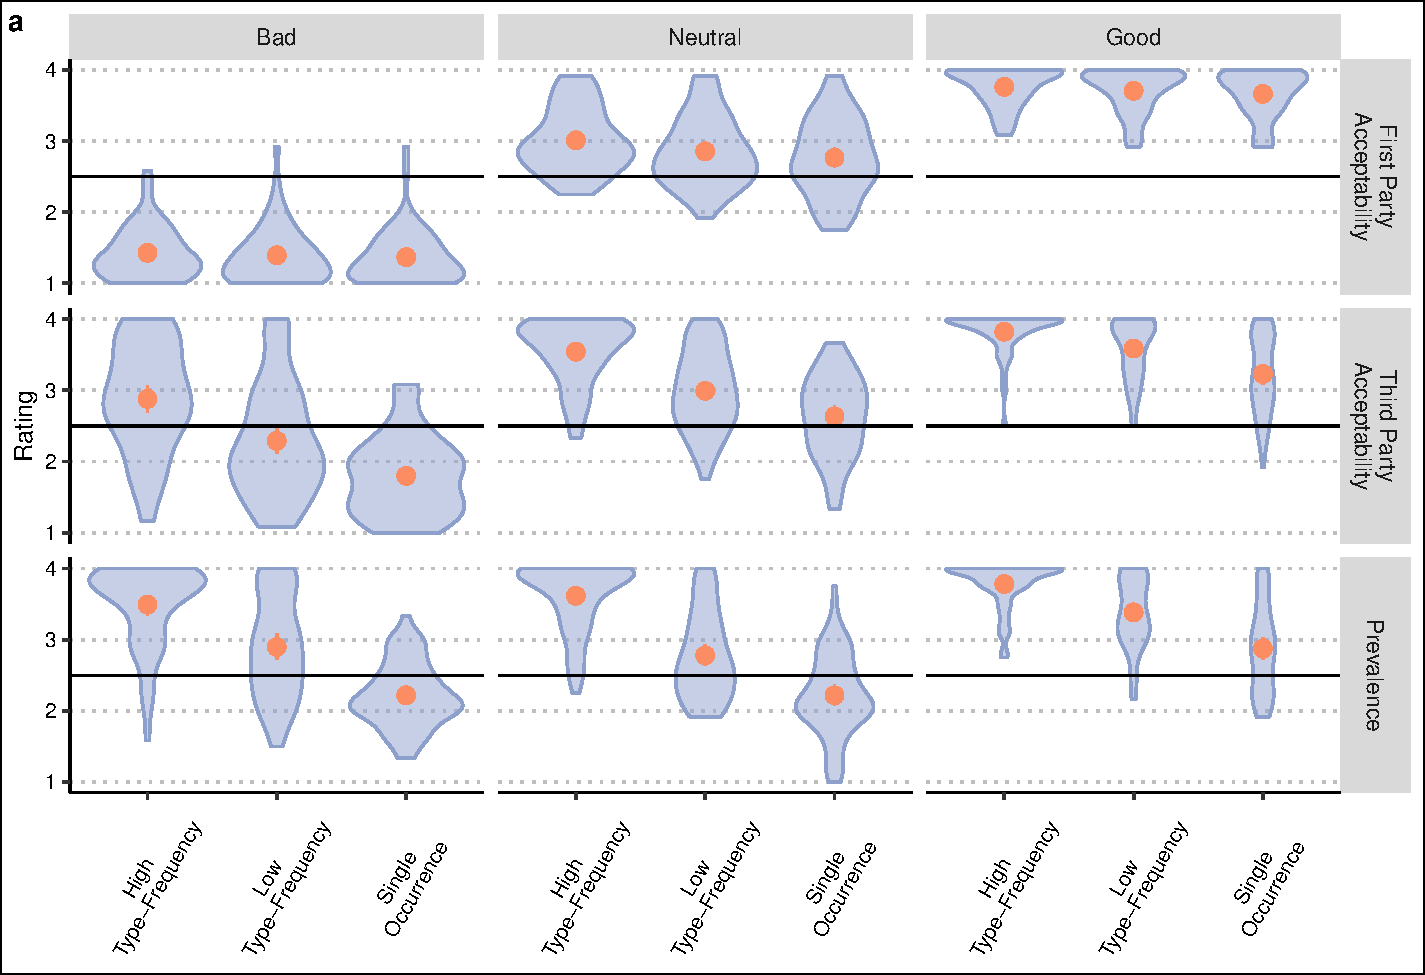
\includegraphics[width=0.8\linewidth]{social_learning_type_token_sequential_results_files/figure-latex/plot-ratings-combined-raw-1} 

}

\caption{Ratings for the combined sample. See Figure~\ref{fig:plot-ratings-raw} for separate results for each sample. The dots, error bars and violin represent the sample average, 95\% bootstrap confidence intervals and the distribution of the individual responses, respectively.}\label{fig:plot-ratings-combined-raw}
\end{figure}

The raw ratings are shown in Figure \ref{fig:plot-ratings-combined-raw} and Table \ref{tab:print-descriptives-ratings-combined-raw2}. As shown in Table \ref{tab:clmm-raw-effects-of-valency-combined2}, a CLMM with a logit link function, including the fixed predictors Valence and Frequency Condition, their interaction, and a random slope for participants, showed that, for both acceptability questions, good deeds were judged more positively than neutral ones, and neutral ones more positively than bad ones. The valence manipulation was thus successful.

\clearpage

\subsection{Comparisons of the High and Low Type-Frequency conditions against the Single-Occurrence condition}\label{comparisons-of-the-high-and-low-type-frequency-conditions-against-the-single-occurrence-condition-3}

I next turn to the question of whether type-frequency or token-frequency affects acceptability and prevalence judgments, using difference scores comparing each frequency condition to the single-occurrence condition.

\subsubsection{Difference scores}\label{difference-scores-2}

\begin{figure}

{\centering 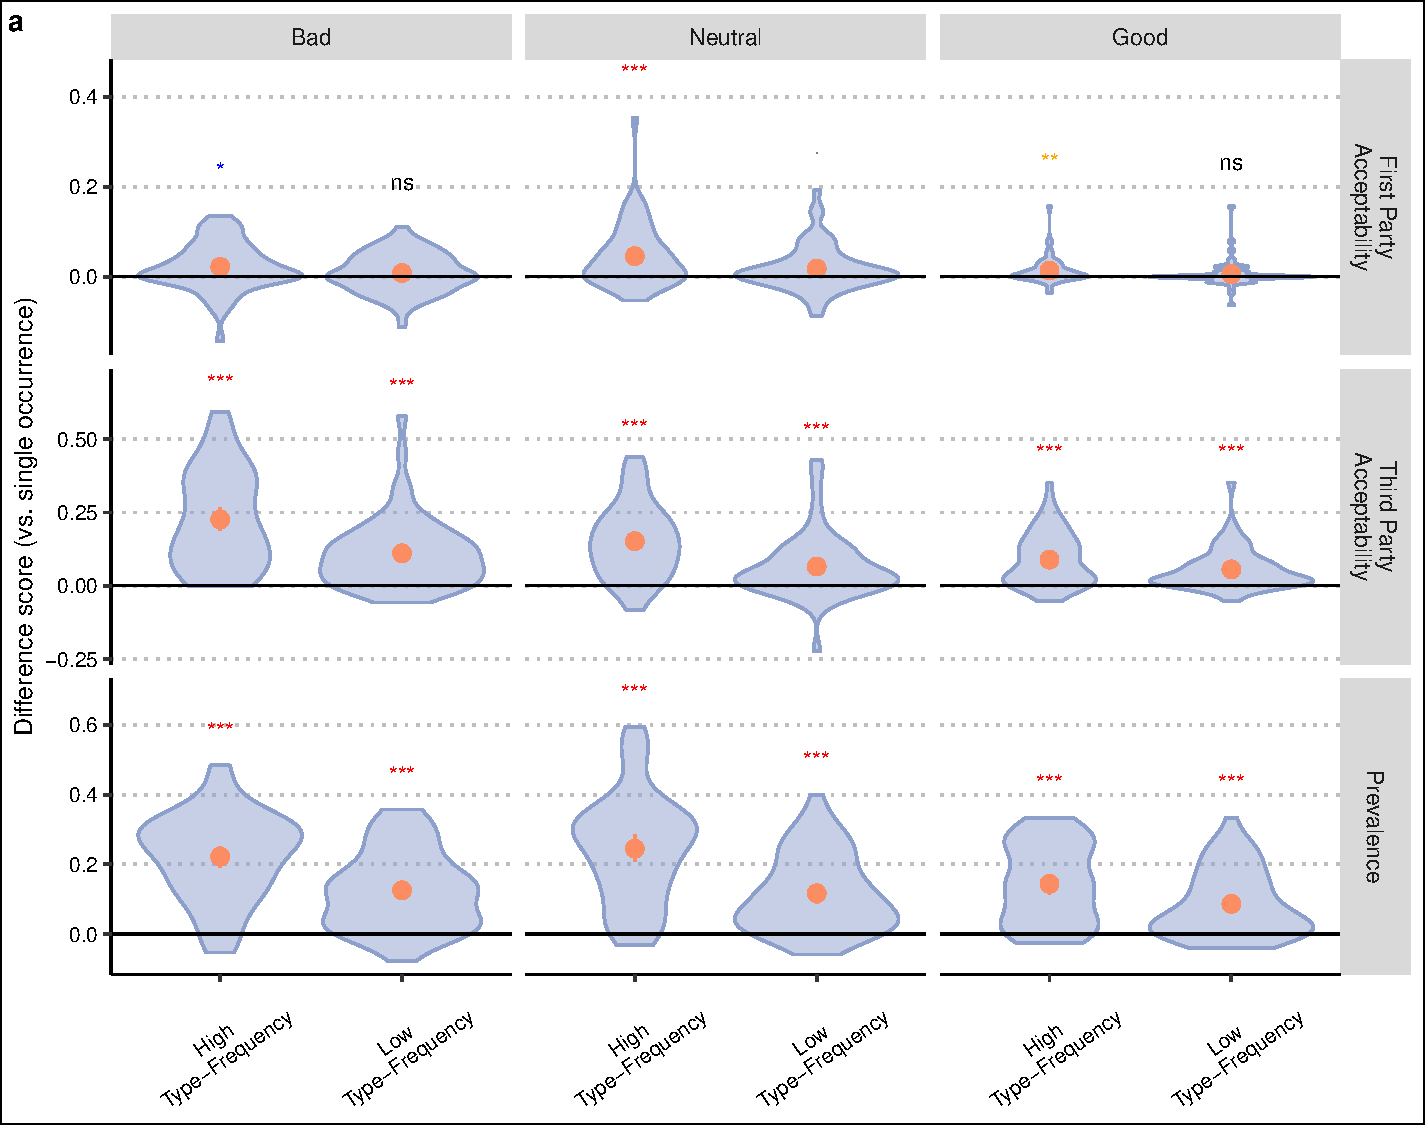
\includegraphics[width=0.8\linewidth]{social_learning_type_token_sequential_results_files/figure-latex/plot-difference-vs-single-combined-raw-1} 

}

\caption{Difference scores against the Single-Occurrence condition for the combined sample ($\frac{\text{High Type-Frequency} - \text{Single-Occurrence}}{\text{High Type-Frequency} + \text{Single-Occurrence}}$ and $\frac{\text{Low Type-Frequency} - \text{Single-Occurrence}}{\text{Low Type-Frequency} + \text{Single-Occurrence}}$). See Figure~\ref{fig:plot-difference-vs-single-raw} for separate results for each sample. The dots, error bars and violin represent the sample average, 95\% bootstrap confidence intervals and the distribution of the individual responses, respectively. Significance codes: *** $p \leq .001$, ** $p \leq .01$, * $p \leq .05$, . $p \leq .10$, ns = not significant.}\label{fig:plot-difference-vs-single-combined-raw}
\end{figure}

The results are shown in Figure \ref{fig:plot-difference-vs-single-combined-raw} and Table \ref{tab:difference-vs-single-raw-combined-print2}. For \emph{first-party acceptability}, ratings in the high type-frequency condition differed reliably from those in the single-occurrence condition for all valences. In contrast, ratings in the low type-frequency condition did not significantly differ from those in the single-occurrence condition; for neutral actions, the difference score was significantly different from zero before correction, but not after correction with the Holm-Bonferroni method. First-party acceptability thus seems primarily driven by type- rather than token-frequency.

To provide evidence for the null hypothesis, I fit two linear models to the first-party acceptability difference scores: one representing the null hypothesis (with the mean fixed at 0) and one representing the alternative hypothesis (with the mean estimated from the data). I then calculated the likelihood of the data under each model, applied corrections for the numbers of parameters using the Bayesian Information Criterion (BIC) and the Akaike Information Criterion (AIC), and computed the likelihood ratio, with values greater than one indicating support for the null hypothesis. As shown in Table \ref{tab:difference-vs-single-raw-combined-print2}, the first-party acceptability difference scores comparing the low type-frequency condition to the single-occurrence condition generally provided weak to moderate evidence in favor of the null hypothesis, suggesting again that first-party acceptability is primarily driven by type-frequency rather than token-frequency.

For both \emph{third-party acceptability} and \emph{prevalence}, ratings in both the high and low type-frequency conditions differed from the single-occurrence condition across all valence conditions, though the difference scores were roughly twice as large for the high type-frequency condition compared to the low type-frequency condition. Both type- and token-frequency thus affect these ratings, though I will demonstrate below that the effect of type-frequency is substantially larger.

\clearpage

\subsubsection{Confirmation with ordinal model}\label{confirmation-with-ordinal-model-2}

I confirmed these results with a series of CLMMs. For each domain (acceptability and prevalence), I included the fixed factor predictors Frequency Condition (High Type-Frequency vs.~Single Occurrence and Low Type-Frequency vs.~Single Occurrence) and Valence (with the reference level set to neutral), as well as a random slope for participants.

\begin{table}
\centering\centering
\caption{\label{tab:clmm-vs-single-occurrence-combined-print-first-party-acceptability}Results from a set of cumulative link mixed models fit on the combined sample for \textbf{First-Party Acceptability}, for the High Type-Frequency vs. Single Occurrence and Low Type-Frequency vs. Single Occurrence contrasts, with fixed factor predictors Frequency Condition and Valence, their interaction, and a random slope for participants. See Table~\ref{tab:clmm-vs-single-occurrence-print} for separate results for each sample. Significance codes: *** $p \leq .001$, ** $p \leq .01$, * $p \leq .05$, . $p \leq .10$, ns = not significant.}
\centering
\begin{tabular}[t]{lrrrrrrl}
\toprule
Parameter & Coefficient & $\mathit{SE}$ & $CI_{\text{low}}$ & $CI_{\text{high}}$ & z & $p$ &  \\
\midrule
\addlinespace[0.3em]
\multicolumn{8}{l}{\textbf{High Type-Frequency vs. Single Occurrence}}\\
\hspace{1em}Valence:bad & -3.384 & 0.264 & -3.902 & -2.866 & -12.806 & 0.000 & ***\\
\hspace{1em}Valence:good & 2.388 & 0.266 & 1.868 & 2.909 & 8.993 & 0.000 & ***\\
\hspace{1em}Freq. Cond:high Type-Freq. & 0.558 & 0.108 & 0.346 & 0.769 & 5.172 & 0.000 & ***\\
\hspace{1em}Valence:bad$\times$Freq. Cond:high Type-Freq. & -0.360 & 0.164 & -0.681 & -0.039 & -2.197 & 0.028 & *\\
\hspace{1em}Valence:good$\times$Freq. Cond:high Type-Freq. & -0.077 & 0.175 & -0.421 & 0.266 & -0.443 & 0.658 & ns\\
\addlinespace[0.3em]
\multicolumn{8}{l}{\textbf{High Type-Frequency vs. Single Occurrence - bad valence only}}\\
\hspace{1em}Freq. Cond:high Type-Freq. & 0.218 & 0.128 & -0.034 & 0.470 & 1.697 & 0.090 & .\\
\addlinespace[0.3em]
\multicolumn{8}{l}{\textbf{High Type-Frequency vs. Single Occurrence - neutral valence only}}\\
\hspace{1em}Freq. Cond:high Type-Freq. & 0.471 & 0.103 & 0.269 & 0.672 & 4.582 & 0.000 & ***\\
\addlinespace[0.3em]
\multicolumn{8}{l}{\textbf{High Type-Frequency vs. Single Occurrence - good valence only}}\\
\hspace{1em}Freq. Cond:high Type-Freq. & 0.546 & 0.144 & 0.264 & 0.828 & 3.791 & 0.000 & ***\\
\addlinespace[0.3em]
\multicolumn{8}{l}{\textbf{Low Type-Frequency vs. Single Occurrence}}\\
\hspace{1em}Valence:bad & -3.466 & 0.277 & -4.010 & -2.923 & -12.508 & 0.000 & ***\\
\hspace{1em}Valence:good & 2.425 & 0.277 & 1.882 & 2.967 & 8.761 & 0.000 & ***\\
\hspace{1em}Freq. Cond:low Type-Freq. & 0.221 & 0.107 & 0.011 & 0.430 & 2.062 & 0.039 & *\\
\hspace{1em}Valence:bad$\times$Freq. Cond:low Type-Freq. & -0.144 & 0.165 & -0.468 & 0.180 & -0.872 & 0.383 & ns\\
\hspace{1em}Valence:good$\times$Freq. Cond:low Type-Freq. & -0.043 & 0.171 & -0.378 & 0.291 & -0.252 & 0.801 & ns\\
\addlinespace[0.3em]
\multicolumn{8}{l}{\textbf{Low Type-Frequency vs. Single Occurrence - bad valence only}}\\
\hspace{1em}Freq. Cond:low Type-Freq. & 0.088 & 0.132 & -0.170 & 0.346 & 0.670 & 0.503 & ns\\
\addlinespace[0.3em]
\multicolumn{8}{l}{\textbf{Low Type-Frequency vs. Single Occurrence - neutral valence only}}\\
\hspace{1em}Freq. Cond:low Type-Freq. & 0.185 & 0.102 & -0.014 & 0.384 & 1.817 & 0.069 & .\\
\addlinespace[0.3em]
\multicolumn{8}{l}{\textbf{Low Type-Frequency vs. Single Occurrence - good valence only}}\\
\hspace{1em}Freq. Cond:low Type-Freq. & 0.199 & 0.138 & -0.072 & 0.470 & 1.440 & 0.150 & ns\\
\bottomrule
\end{tabular}
\end{table}
\begin{table}
\centering\centering
\caption{\label{tab:clmm-vs-single-occurrence-combined-print-third-party-acceptability}Results from a set of cumulative link mixed models fit on the combined sample for \textbf{Third-Party Acceptability}, for the High Type-Frequency vs. Single Occurrence and Low Type-Frequency vs. Single Occurrence contrasts, with fixed factor predictors Frequency Condition and Valence, their interaction, and a random slope for participants. For the Low Type-Frequency vs. Single Occurrence contrast, the Valence $\times$ Frequency Condition interaction was omitted (additive model used) due to complete separation encountered in one of the individual samples (zero observations at the lowest rating for good actions). See Table~\ref{tab:clmm-vs-single-occurrence-print} for separate results for each sample. Significance codes: *** $p \leq .001$, ** $p \leq .01$, * $p \leq .05$, . $p \leq .10$, ns = not significant.}
\centering
\begin{tabular}[t]{lrrrrrrl}
\toprule
Parameter & Coefficient & $\mathit{SE}$ & $CI_{\text{low}}$ & $CI_{\text{high}}$ & z & $p$ &  \\
\midrule
\addlinespace[0.3em]
\multicolumn{8}{l}{\textbf{High Type-Frequency vs. Single Occurrence}}\\
\hspace{1em}Valence:bad & -2.041 & 0.267 & -2.565 & -1.518 & -7.646 & 0.000 & ***\\
\hspace{1em}Valence:good & 1.561 & 0.268 & 1.035 & 2.087 & 5.818 & 0.000 & ***\\
\hspace{1em}Freq. Cond:high Type-Freq. & 2.614 & 0.124 & 2.371 & 2.857 & 21.089 & 0.000 & ***\\
\hspace{1em}Valence:bad$\times$Freq. Cond:high Type-Freq. & 0.043 & 0.159 & -0.269 & 0.355 & 0.271 & 0.786 & ns\\
\hspace{1em}Valence:good$\times$Freq. Cond:high Type-Freq. & -0.157 & 0.184 & -0.517 & 0.203 & -0.856 & 0.392 & ns\\
\addlinespace[0.3em]
\multicolumn{8}{l}{\textbf{High Type-Frequency vs. Single Occurrence - bad valence only}}\\
\hspace{1em}Freq. Cond:high Type-Freq. & 2.852 & 0.131 & 2.595 & 3.109 & 21.759 & 0.000 & ***\\
\addlinespace[0.3em]
\multicolumn{8}{l}{\textbf{High Type-Frequency vs. Single Occurrence - neutral valence only}}\\
\hspace{1em}Freq. Cond:high Type-Freq. & 2.257 & 0.124 & 2.014 & 2.500 & 18.228 & 0.000 & ***\\
\addlinespace[0.3em]
\multicolumn{8}{l}{\textbf{High Type-Frequency vs. Single Occurrence - good valence only}}\\
\hspace{1em}Freq. Cond:high Type-Freq. & 2.709 & 0.160 & 2.394 & 3.023 & 16.878 & 0.000 & ***\\
\addlinespace[0.3em]
\multicolumn{8}{l}{\textbf{Low Type-Frequency vs. Single Occurrence}}\\
\hspace{1em}Valence:bad & -2.110 & 0.072 & -2.250 & -1.969 & -29.429 & 0.000 & ***\\
\hspace{1em}Valence:good & 1.800 & 0.175 & 1.457 & 2.143 & 10.284 & 0.000 & ***\\
\hspace{1em}Freq. Cond:low Type-Freq. & 1.169 & 0.048 & 1.075 & 1.263 & 24.335 & 0.000 & ***\\
\addlinespace[0.3em]
\multicolumn{8}{l}{\textbf{Low Type-Frequency vs. Single Occurrence - bad valence only}}\\
\hspace{1em}Freq. Cond:low Type-Freq. & 1.423 & 0.004 & 1.416 & 1.431 & 385.758 & 0.000 & ***\\
\addlinespace[0.3em]
\multicolumn{8}{l}{\textbf{Low Type-Frequency vs. Single Occurrence - neutral valence only}}\\
\hspace{1em}Freq. Cond:low Type-Freq. & 0.812 & 0.104 & 0.608 & 1.016 & 7.806 & 0.000 & ***\\
\addlinespace[0.3em]
\multicolumn{8}{l}{\textbf{Low Type-Frequency vs. Single Occurrence - good valence only}}\\
\hspace{1em}Freq. Cond:low Type-Freq. & 1.422 & 0.130 & 1.167 & 1.678 & 10.917 & 0.000 & ***\\
\bottomrule
\end{tabular}
\end{table}
\begin{table}
\centering\centering
\caption{\label{tab:clmm-vs-single-occurrence-combined-print-prevalence}Results from a set of cumulative link mixed models fit on the combined sample for \textbf{Prevalence}, for the High Type-Frequency vs. Single Occurrence and Low Type-Frequency vs. Single Occurrence contrasts, with fixed factor predictors Frequency Condition and Valence, their interaction, and a random slope for participants. See Table~\ref{tab:clmm-vs-single-occurrence-print} for separate results for each sample. Significance codes: *** $p \leq .001$, ** $p \leq .01$, * $p \leq .05$, . $p \leq .10$, ns = not significant.}
\centering
\begin{tabular}[t]{lrrrrrrl}
\toprule
Parameter & Coefficient & $\mathit{SE}$ & $CI_{\text{low}}$ & $CI_{\text{high}}$ & z & $p$ &  \\
\midrule
\addlinespace[0.3em]
\multicolumn{8}{l}{\textbf{High Type-Frequency vs. Single Occurrence}}\\
\hspace{1em}Valence:bad & 0.053 & 0.258 & -0.452 & 0.558 & 0.204 & 0.838 & ns\\
\hspace{1em}Valence:good & 1.883 & 0.262 & 1.370 & 2.395 & 7.199 & 0.000 & ***\\
\hspace{1em}Freq. Cond:high Type-Freq. & 4.298 & 0.142 & 4.019 & 4.577 & 30.212 & 0.000 & ***\\
\hspace{1em}Valence:bad$\times$Freq. Cond:high Type-Freq. & -0.709 & 0.168 & -1.037 & -0.380 & -4.230 & 0.000 & ***\\
\hspace{1em}Valence:good$\times$Freq. Cond:high Type-Freq. & -1.076 & 0.185 & -1.437 & -0.714 & -5.826 & 0.000 & ***\\
\addlinespace[0.3em]
\multicolumn{8}{l}{\textbf{High Type-Frequency vs. Single Occurrence - bad valence only}}\\
\hspace{1em}Freq. Cond:high Type-Freq. & 3.862 & 0.156 & 3.556 & 4.168 & 24.763 & 0.000 & ***\\
\addlinespace[0.3em]
\multicolumn{8}{l}{\textbf{High Type-Frequency vs. Single Occurrence - neutral valence only}}\\
\hspace{1em}Freq. Cond:high Type-Freq. & 3.660 & 0.152 & 3.362 & 3.959 & 24.012 & 0.000 & ***\\
\addlinespace[0.3em]
\multicolumn{8}{l}{\textbf{High Type-Frequency vs. Single Occurrence - good valence only}}\\
\hspace{1em}Freq. Cond:high Type-Freq. & 3.537 & 0.167 & 3.210 & 3.864 & 21.191 & 0.000 & ***\\
\addlinespace[0.3em]
\multicolumn{8}{l}{\textbf{Low Type-Frequency vs. Single Occurrence}}\\
\hspace{1em}Valence:bad & 0.015 & 0.330 & -0.632 & 0.661 & 0.044 & 0.965 & ns\\
\hspace{1em}Valence:good & 2.170 & 0.334 & 1.515 & 2.825 & 6.496 & 0.000 & ***\\
\hspace{1em}Freq. Cond:low Type-Freq. & 1.798 & 0.116 & 1.571 & 2.025 & 15.502 & 0.000 & ***\\
\hspace{1em}Valence:bad$\times$Freq. Cond:low Type-Freq. & 0.283 & 0.156 & -0.022 & 0.588 & 1.819 & 0.069 & .\\
\hspace{1em}Valence:good$\times$Freq. Cond:low Type-Freq. & -0.188 & 0.160 & -0.501 & 0.125 & -1.176 & 0.239 & ns\\
\addlinespace[0.3em]
\multicolumn{8}{l}{\textbf{Low Type-Frequency vs. Single Occurrence - bad valence only}}\\
\hspace{1em}Freq. Cond:low Type-Freq. & 2.166 & 0.126 & 1.919 & 2.413 & 17.214 & 0.000 & ***\\
\addlinespace[0.3em]
\multicolumn{8}{l}{\textbf{Low Type-Frequency vs. Single Occurrence - neutral valence only}}\\
\hspace{1em}Freq. Cond:low Type-Freq. & 1.611 & 0.004 & 1.603 & 1.619 & 401.104 & 0.000 & ***\\
\addlinespace[0.3em]
\multicolumn{8}{l}{\textbf{Low Type-Frequency vs. Single Occurrence - good valence only}}\\
\hspace{1em}Freq. Cond:low Type-Freq. & 1.778 & 0.126 & 1.531 & 2.024 & 14.126 & 0.000 & ***\\
\bottomrule
\end{tabular}
\end{table}

For \emph{first-party acceptability}, Table \ref{tab:clmm-vs-single-occurrence-combined-print-first-party-acceptability} shows that ratings differed significantly from the single-occurrence condition in both the high type-frequency condition and the low type-frequency condition, though the coefficient in the high type-frequency condition was more than twice as high. This suggests that first-party acceptability is primarily driven by type-frequency. For the high type-frequency vs.~single occurrence contrast, there was an interaction with valence. Valence-specific CLMMs suggested that the effect of the difference between the high type-frequency condition and the single-occurrence condition was reduced and only marginal for bad actions. In contrast, the contrast between the low type-frequency condition and the single-occurrence condition was not significant for bad or good actions, and only marginal for neutral actions.

For \emph{third-party acceptability} (Table \ref{tab:clmm-vs-single-occurrence-combined-print-third-party-acceptability}), both the high and low type-frequency conditions differed from the single-occurrence condition. However, the parameter estimate was approximately two times greater for the high type-frequency condition than for the low type-frequency condition.

For \emph{prevalence} (Table \ref{tab:clmm-vs-single-occurrence-combined-print-prevalence}), both the high and low type-frequency conditions differed from the single-occurrence condition. However, the parameter estimates were approximately 2.3 times greater for the high type-frequency condition than for the low type-frequency condition.

\subsection{Comparisons of the High and Low Type-Frequency conditions}\label{comparisons-of-the-high-and-low-type-frequency-conditions-3}

I now turn to the question of whether type and token frequency affect ratings differentially. I first address this question using difference scores, and then confirm these results using a CLMM.

\subsubsection{Difference scores}\label{difference-scores-3}

\begin{figure}

{\centering 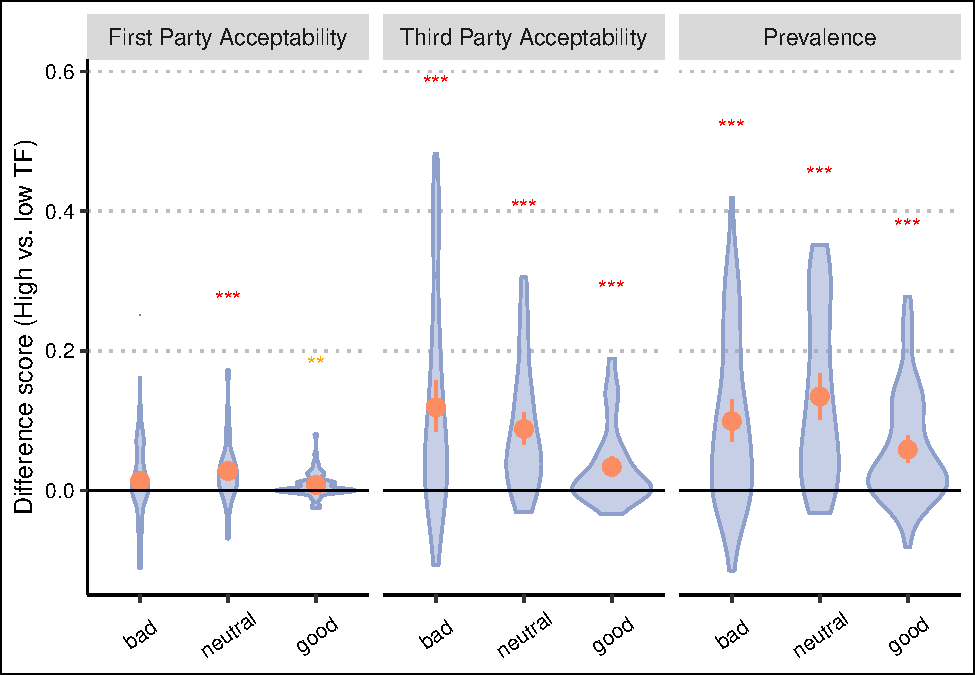
\includegraphics[width=0.8\linewidth]{social_learning_type_token_sequential_results_files/figure-latex/plot-difference-high-vs-low-type-frequency-combined-raw-1} 

}

\caption{Difference scores comparing the High and Low Type-Frequency Conditions for the combined sample ($\frac{\text{High Type-Frequency} - \text{Low Type-Frequency}}{\text{High Type-Frequency} + \text{Low Type-Frequency}}$). See Figure~\ref{fig:plot-difference-high-vs-low-type-frequency-raw} for separate results for each sample. The dots, error bars and violin represent the sample average, 95\% bootstrap confidence intervals and the distribution of the individual responses, respectively. Significance codes: *** $p \leq .001$, ** $p \leq .01$, * $p \leq .05$, . $p \leq .10$, ns = not significant.}\label{fig:plot-difference-high-vs-low-type-frequency-combined-raw}
\end{figure}

The results are shown in Figure \ref{fig:plot-difference-high-vs-low-type-frequency-combined-raw} and Table \ref{tab:difference-high-vs-low-type-frequency-combined-print2}. For first-party acceptability, the difference scores were significantly greater than zero for neutral and good actions; for bad actions, the effect was only marginal after Holm-Bonferroni correction. First-party acceptability ratings thus increase when the type frequency of an action is increased, even when the frequency of occurrence is held constant.

For \emph{third-party acceptability} and \emph{prevalence}, the difference scores were significantly greater than zero for all valence conditions, showing again that type-frequency has an effect over and above frequency of occurrence.

\clearpage

\subsubsection{Confirmation with ordinal model}\label{confirmation-with-ordinal-model-3}

I confirmed these results with a series of CLMMs. For each domain, I fitted a model including the fixed factor predictors Frequency Condition (High Type-Frequency vs.~Low Type-Frequency) and Valence, with the reference level set to neutral.

\begin{table}
\centering\centering
\caption{\label{tab:clmm-high-vs-low-type-frequency-combined-print-first-party-acceptability}Results from a set of cumulative link mixed models for the combined sample for \textbf{First-Party Acceptability}, contrasting the High Type-Frequency condition with the Low Type-Frequency condition, with fixed factor predictors Valence, Frequency Condition, and their interaction, as well as a random slope for participants. See Table~\ref{tab:clmm-high-vs-low-type-frequency-print} for separate results for each sample. Significance codes: *** $p \leq .001$, ** $p \leq .01$, * $p \leq .05$, . $p \leq .10$, ns = not significant.}
\centering
\begin{tabular}[t]{lrrrrrrl}
\toprule
Parameter & Coefficient & $\mathit{SE}$ & $CI_{\text{low}}$ & $CI_{\text{high}}$ & z & $p$ &  \\
\midrule
\addlinespace[0.3em]
\multicolumn{8}{l}{\textbf{High Type-Frequency vs. Low Type-Frequency}}\\
\hspace{1em}Valence:bad & -3.623 & 0.272 & -4.155 & -3.090 & -13.336 & 0.000 & ***\\
\hspace{1em}Valence:good & 2.373 & 0.275 & 1.835 & 2.912 & 8.638 & 0.000 & ***\\
\hspace{1em}Freq. Cond:high Type-Freq. & 0.338 & 0.108 & 0.126 & 0.550 & 3.129 & 0.002 & **\\
\hspace{1em}Valence:bad$\times$Freq. Cond:high Type-Freq. & -0.211 & 0.164 & -0.532 & 0.111 & -1.285 & 0.199 & ns\\
\hspace{1em}Valence:good$\times$Freq. Cond:high Type-Freq. & -0.030 & 0.178 & -0.379 & 0.319 & -0.169 & 0.866 & ns\\
\bottomrule
\end{tabular}
\end{table}
\begin{table}
\centering\centering
\caption{\label{tab:clmm-high-vs-low-type-frequency-combined-print-third-party-acceptability}Results from a set of cumulative link mixed models for the combined sample for \textbf{Third-Party Acceptability}, contrasting the High Type-Frequency condition with the Low Type-Frequency condition, with fixed factor predictors Valence, Frequency Condition, and their interaction, as well as a random slope for participants. See Table~\ref{tab:clmm-high-vs-low-type-frequency-print} for separate results for each sample. Significance codes: *** $p \leq .001$, ** $p \leq .01$, * $p \leq .05$, . $p \leq .10$, ns = not significant.}
\centering
\begin{tabular}[t]{lrrrrrrl}
\toprule
Parameter & Coefficient & $\mathit{SE}$ & $CI_{\text{low}}$ & $CI_{\text{high}}$ & z & $p$ &  \\
\midrule
\addlinespace[0.3em]
\multicolumn{8}{l}{\textbf{High Type-Frequency vs. Low Type-Frequency}}\\
\hspace{1em}Valence:bad & -1.698 & 0.335 & -2.355 & -1.041 & -5.06 & 0.000 & ***\\
\hspace{1em}Valence:good & 1.959 & 0.345 & 1.283 & 2.635 & 5.68 & 0.000 & ***\\
\hspace{1em}Freq. Cond:high Type-Freq. & 1.823 & 0.124 & 1.580 & 2.066 & 14.70 & 0.000 & ***\\
\hspace{1em}Valence:bad$\times$Freq. Cond:high Type-Freq. & -0.313 & 0.161 & -0.629 & 0.003 & -1.94 & 0.053 & .\\
\hspace{1em}Valence:good$\times$Freq. Cond:high Type-Freq. & -0.437 & 0.192 & -0.814 & -0.060 & -2.27 & 0.023 & *\\
\addlinespace[0.3em]
\multicolumn{8}{l}{\textbf{High Type-Frequency vs. Low Type-Frequency - bad valence only}}\\
\hspace{1em}Freq. Cond:high Type-Freq. & 1.597 & 0.116 & 1.370 & 1.823 & 13.80 & 0.000 & ***\\
\addlinespace[0.3em]
\multicolumn{8}{l}{\textbf{High Type-Frequency vs. Low Type-Frequency - neutral valence only}}\\
\hspace{1em}Freq. Cond:high Type-Freq. & 1.598 & 0.122 & 1.360 & 1.837 & 13.14 & 0.000 & ***\\
\addlinespace[0.3em]
\multicolumn{8}{l}{\textbf{High Type-Frequency vs. Low Type-Frequency - good valence only}}\\
\hspace{1em}Freq. Cond:high Type-Freq. & 1.522 & 0.158 & 1.213 & 1.831 & 9.64 & 0.000 & ***\\
\bottomrule
\end{tabular}
\end{table}
\begin{table}
\centering\centering
\caption{\label{tab:clmm-high-vs-low-type-frequency-combined-print-prevalence}Results from a set of cumulative link mixed models for the combined sample for \textbf{Prevalence}, contrasting the High Type-Frequency condition with the Low Type-Frequency condition, with fixed factor predictors Valence, Frequency Condition, and their interaction, as well as a random slope for participants. See Table~\ref{tab:clmm-high-vs-low-type-frequency-print} for separate results for each sample. Significance codes: *** $p \leq .001$, ** $p \leq .01$, * $p \leq .05$, . $p \leq .10$, ns = not significant.}
\centering
\begin{tabular}[t]{lrrrrrrl}
\toprule
Parameter & Coefficient & $\mathit{SE}$ & $CI_{\text{low}}$ & $CI_{\text{high}}$ & z & $p$ &  \\
\midrule
\addlinespace[0.3em]
\multicolumn{8}{l}{\textbf{High Type-Frequency vs. Low Type-Frequency}}\\
\hspace{1em}Valence:bad & 0.381 & 0.346 & -0.296 & 1.059 & 1.10 & 0.27 & ns\\
\hspace{1em}Valence:good & 1.874 & 0.353 & 1.182 & 2.565 & 5.31 & 0.00 & ***\\
\hspace{1em}Freq. Cond:high Type-Freq. & 2.886 & 0.133 & 2.625 & 3.147 & 21.67 & 0.00 & ***\\
\hspace{1em}Valence:bad$\times$Freq. Cond:high Type-Freq. & -0.858 & 0.172 & -1.196 & -0.520 & -4.98 & 0.00 & ***\\
\hspace{1em}Valence:good$\times$Freq. Cond:high Type-Freq. & -1.050 & 0.187 & -1.416 & -0.684 & -5.62 & 0.00 & ***\\
\addlinespace[0.3em]
\multicolumn{8}{l}{\textbf{High Type-Frequency vs. Low Type-Frequency - bad valence only}}\\
\hspace{1em}Freq. Cond:high Type-Freq. & 2.044 & 0.131 & 1.788 & 2.299 & 15.65 & 0.00 & ***\\
\addlinespace[0.3em]
\multicolumn{8}{l}{\textbf{High Type-Frequency vs. Low Type-Frequency - neutral valence only}}\\
\hspace{1em}Freq. Cond:high Type-Freq. & 2.593 & 0.138 & 2.322 & 2.863 & 18.78 & 0.00 & ***\\
\addlinespace[0.3em]
\multicolumn{8}{l}{\textbf{High Type-Frequency vs. Low Type-Frequency - good valence only}}\\
\hspace{1em}Freq. Cond:high Type-Freq. & 2.024 & 0.149 & 1.733 & 2.315 & 13.62 & 0.00 & ***\\
\bottomrule
\end{tabular}
\end{table}

For first-party acceptability (Table \ref{tab:clmm-high-vs-low-type-frequency-combined-print-first-party-acceptability}), third-party acceptability (Table \ref{tab:clmm-high-vs-low-type-frequency-combined-print-third-party-acceptability}), and prevalence (Table \ref{tab:clmm-high-vs-low-type-frequency-combined-print-prevalence}), ratings in the high type-frequency condition were higher than those in the low type-frequency condition.

I also observed main effects of valence, showing that good actions were rated higher than neutral ones, while neutral ones were rated higher than bad ones (except for prevalence ratings, where the latter two conditions did not differ).
These results thus mirror those of the difference scores above.

For third-party acceptability and prevalence, an interaction between Frequency Condition and Valence suggested that the effect of Frequency Condition was somewhat reduced for bad and good actions compared to neutral actions, though the effect was significant for all valences.

\clearpage

\subsection{Alternative analyses}\label{alternative-analyses-1}

In\textasciitilde{}\ref{app:alternative-analyses}, I report two alternative sets of analyses in addition to the difference score analyses and the CLMMs. First, I fit a series of generalized linear mixed models (GLMMs) using binarized responses, where ratings of 1 or 2 were coded as ``unacceptable'' and ratings of 3 or 4 as ``acceptable.'' These models compared both the high type-frequency (TF) and low TF conditions to the single-occurrence condition, as well as directly compared the high TF and low TF conditions. Second, I conducted a set of equivalent mixed ANOVAs to assess the robustness of the results. The results were largely consistent with those of the main analyses.

\clearpage

\section{Appendix}\label{appendix-1}

\section{Descriptives}\label{descriptives-1}

\subsection{Raw ratings}\label{raw-ratings-3}

\begin{longtable}[t]{lrrrrrl}
\caption{\label{tab:print-descriptives-ratings-combined-raw2}Descriptives for the raw ratings for the combined sample. The p value reflects a Wilcoxon test against the scale midpoint of 2.5. See Table~\ref{tab:print-descriptives-ratings-raw2} for separate results for each sample. Significance codes: *** $p \leq .001$, ** $p \leq .01$, * $p \leq .05$, . $p \leq .10$, ns = not significant.}\\
\toprule
 & N & M & SE & Cohen's d & p &  \\
\midrule
\endfirsthead
\caption[]{\label{tab:print-descriptives-ratings-combined-raw2}Descriptives for the raw ratings for the combined sample. The p value reflects a Wilcoxon test against the scale midpoint of 2.5. See Table~\ref{tab:print-descriptives-ratings-raw2} for separate results for each sample. Significance codes: *** $p \leq .001$, ** $p \leq .01$, * $p \leq .05$, . $p \leq .10$, ns = not significant. \textit{(continued)}}\\
\toprule
 & N & M & SE & Cohen's d & p &  \\
\midrule
\endhead

\endfoot
\bottomrule
\endlastfoot
\addlinespace[0.3em]
\multicolumn{7}{l}{\textbf{First Party Acceptability - bad}}\\
\hspace{1em}High Type-Frequency & 58 & 1.43 & 0.049 & 3.89 & 0.000 & ***\\
\hspace{1em}Low Type-Frequency & 58 & 1.40 & 0.052 & 3.53 & 0.000 & ***\\
\hspace{1em}Single Occurrence & 58 & 1.37 & 0.051 & 3.58 & 0.000 & ***\\
\addlinespace[0.3em]
\multicolumn{7}{l}{\textbf{First Party Acceptability - neutral}}\\
\hspace{1em}High Type-Frequency & 56 & 3.01 & 0.060 & 6.71 & 0.000 & ***\\
\hspace{1em}Low Type-Frequency & 56 & 2.86 & 0.066 & 5.85 & 0.000 & ***\\
\hspace{1em}Single Occurrence & 56 & 2.77 & 0.073 & 5.13 & 0.001 & **\\
\addlinespace[0.3em]
\multicolumn{7}{l}{\textbf{First Party Acceptability - good}}\\
\hspace{1em}High Type-Frequency & 57 & 3.76 & 0.036 & 13.85 & 0.000 & ***\\
\hspace{1em}Low Type-Frequency & 57 & 3.71 & 0.042 & 11.91 & 0.000 & ***\\
\hspace{1em}Single Occurrence & 57 & 3.66 & 0.044 & 11.15 & 0.000 & ***\\
\addlinespace[0.3em]
\multicolumn{7}{l}{\textbf{Third Party Acceptability - bad}}\\
\hspace{1em}High Type-Frequency & 58 & 2.88 & 0.100 & 3.81 & 0.001 & ***\\
\hspace{1em}Low Type-Frequency & 58 & 2.29 & 0.105 & 2.88 & 0.032 & *\\
\hspace{1em}Single Occurrence & 58 & 1.80 & 0.073 & 3.27 & 0.000 & ***\\
\addlinespace[0.3em]
\multicolumn{7}{l}{\textbf{Third Party Acceptability - neutral}}\\
\hspace{1em}High Type-Frequency & 56 & 3.54 & 0.060 & 7.91 & 0.000 & ***\\
\hspace{1em}Low Type-Frequency & 56 & 2.99 & 0.076 & 5.34 & 0.000 & ***\\
\hspace{1em}Single Occurrence & 56 & 2.63 & 0.076 & 4.69 & 0.074 & .\\
\addlinespace[0.3em]
\multicolumn{7}{l}{\textbf{Third Party Acceptability - good}}\\
\hspace{1em}High Type-Frequency & 57 & 3.83 & 0.038 & 13.31 & 0.000 & ***\\
\hspace{1em}Low Type-Frequency & 57 & 3.59 & 0.055 & 8.65 & 0.000 & ***\\
\hspace{1em}Single Occurrence & 57 & 3.23 & 0.073 & 5.88 & 0.000 & ***\\
\addlinespace[0.3em]
\multicolumn{7}{l}{\textbf{Prevalence - bad}}\\
\hspace{1em}High Type-Frequency & 58 & 3.49 & 0.075 & 6.17 & 0.000 & ***\\
\hspace{1em}Low Type-Frequency & 58 & 2.90 & 0.096 & 4.02 & 0.000 & ***\\
\hspace{1em}Single Occurrence & 58 & 2.22 & 0.060 & 4.89 & 0.000 & ***\\
\addlinespace[0.3em]
\multicolumn{7}{l}{\textbf{Prevalence - neutral}}\\
\hspace{1em}High Type-Frequency & 56 & 3.62 & 0.064 & 7.57 & 0.000 & ***\\
\hspace{1em}Low Type-Frequency & 56 & 2.78 & 0.081 & 4.60 & 0.005 & **\\
\hspace{1em}Single Occurrence & 56 & 2.22 & 0.077 & 3.88 & 0.001 & ***\\
\addlinespace[0.3em]
\multicolumn{7}{l}{\textbf{Prevalence - good}}\\
\hspace{1em}High Type-Frequency & 57 & 3.78 & 0.042 & 12.09 & 0.000 & ***\\
\hspace{1em}Low Type-Frequency & 57 & 3.38 & 0.065 & 6.98 & 0.000 & ***\\
\hspace{1em}Single Occurrence & 57 & 2.87 & 0.082 & 4.66 & 0.000 & ***\\*
\end{longtable}

First-party and third-party acceptability ratings were below the midpoint of 2.5 for bad actions, and above the midpoint for neutral and good actions.

Prevalence ratings showed a more complex relationship to valence. For bad and neutral actions, high- and low-type-frequency actions showed ratings above the midpoints, while single-occurrence actions showed ratings below the midpoint. For good actions, ratings were above the midpoint for all frequency conditions.

\begin{longtable}[t]{lrrrrrrl}
\caption{\label{tab:clmm-raw-effects-of-valency-combined2}Results from a set of cumulative link mixed models for the combined sample, fit separately for each domain (first-party acceptability and third-party acceptability), with the fixed factor predictors valence and frequency condition as well as their interaction, as well as a random slope for participants. See Table~\ref{tab:clmm-raw-effects-of-valency2} for separate results for each sample. Only the main effect of valence is shown. Significance codes: *** $p \leq .001$, ** $p \leq .01$, * $p \leq .05$, . $p \leq .10$, ns = not significant.}\\
\toprule
Parameter & Coefficient & $\mathit{SE}$ & $CI_{\text{low}}$ & $CI_{\text{high}}$ & z & $p$ &  \\
\midrule
\endfirsthead
\caption[]{\label{tab:clmm-raw-effects-of-valency-combined2}Results from a set of cumulative link mixed models for the combined sample, fit separately for each domain (first-party acceptability and third-party acceptability), with the fixed factor predictors valence and frequency condition as well as their interaction, as well as a random slope for participants. See Table~\ref{tab:clmm-raw-effects-of-valency2} for separate results for each sample. Only the main effect of valence is shown. Significance codes: *** $p \leq .001$, ** $p \leq .01$, * $p \leq .05$, . $p \leq .10$, ns = not significant. \textit{(continued)}}\\
\toprule
Parameter & Coefficient & $\mathit{SE}$ & $CI_{\text{low}}$ & $CI_{\text{high}}$ & z & $p$ &  \\
\midrule
\endhead

\endfoot
\bottomrule
\endlastfoot
\addlinespace[0.3em]
\multicolumn{8}{l}{\textbf{First Party Acceptability}}\\
\hspace{1em}Valence:bad & -3.84 & 0.276 & -4.38 & -3.30 & -13.89 & 0 & ***\\
\hspace{1em}Valence:good & 2.37 & 0.283 & 1.81 & 2.92 & 8.38 & 0 & ***\\
\addlinespace[0.3em]
\multicolumn{8}{l}{\textbf{Third Party Acceptability}}\\
\hspace{1em}Valence:bad & -2.00 & 0.288 & -2.57 & -1.44 & -6.96 & 0 & ***\\
\hspace{1em}Valence:good & 1.46 & 0.306 & 0.86 & 2.06 & 4.77 & 0 & ***\\*
\end{longtable}

As shown in Table \ref{tab:clmm-raw-effects-of-valency-combined2}, acceptability ratings were higher for good actions than for neutral actions, and for neutral actions than for bad actions.

\clearpage

\subsection{Comparisons of the High and Low Type-Frequency conditions against the Single-Occurrence condition}\label{comparisons-of-the-high-and-low-type-frequency-conditions-against-the-single-occurrence-condition-4}

\begin{longtable}[t]{llrrrrrrlrr}
\caption{\label{tab:difference-vs-single-raw-combined-print2}Descriptives for the difference scores against the Single-Occurrence condition for the combined sample ($\frac{\text{High Type-Frequency} - \text{Single-Occurrence}}{\text{High Type-Frequency} + \text{Single-Occurrence}}$ and $\frac{\text{Low Type-Frequency} - \text{Single-Occurrence}}{\text{Low Type-Frequency} + \text{Single-Occurrence}}$). The p-value reflects a Wilcoxon test against zero. $p_{\scriptsize{hb}}$ reflects the Holm-Bonferroni corrected p-value. See Table~\ref{tab:difference-vs-single-raw-print2} for separate results for each sample. The likelihood ratios $LR_{01,\text{BIC}}$ and $LR_{01,\text{AIC}}$ reflect the evidence in favor of the null hypothesis, after correction using the Bayesian Information Criterion and the Akaike Information Criterion, respectively. Different participants took part in each of the valence conditions. Significance codes: *** $p \leq .001$, ** $p \leq .01$, * $p \leq .05$, . $p \leq .10$, ns = not significant.}\\
\toprule
Valence & Frequency Condition & N & $M$ & $\mathit{SE}$ & Cohen's $d$ & $p$ & $p_{\text{hb}}$ &   & lr01.bic & lr01.aic\\
\midrule
\endfirsthead
\caption[]{\label{tab:difference-vs-single-raw-combined-print2}Descriptives for the difference scores against the Single-Occurrence condition for the combined sample ($\frac{\text{High Type-Frequency} - \text{Single-Occurrence}}{\text{High Type-Frequency} + \text{Single-Occurrence}}$ and $\frac{\text{Low Type-Frequency} - \text{Single-Occurrence}}{\text{Low Type-Frequency} + \text{Single-Occurrence}}$). The p-value reflects a Wilcoxon test against zero. $p_{\scriptsize{hb}}$ reflects the Holm-Bonferroni corrected p-value. See Table~\ref{tab:difference-vs-single-raw-print2} for separate results for each sample. The likelihood ratios $LR_{01,\text{BIC}}$ and $LR_{01,\text{AIC}}$ reflect the evidence in favor of the null hypothesis, after correction using the Bayesian Information Criterion and the Akaike Information Criterion, respectively. Different participants took part in each of the valence conditions. Significance codes: *** $p \leq .001$, ** $p \leq .01$, * $p \leq .05$, . $p \leq .10$, ns = not significant. \textit{(continued)}}\\
\toprule
Valence & Frequency Condition & N & $M$ & $\mathit{SE}$ & Cohen's $d$ & $p$ & $p_{\text{hb}}$ &   & lr01.bic & lr01.aic\\
\midrule
\endhead

\endfoot
\bottomrule
\endlastfoot
\addlinespace[0.3em]
\multicolumn{11}{l}{\textbf{First Party Acceptability}}\\
\hspace{1em}bad & High Type-Frequency & 58 & 0.022 & 0.007 & 0.418 & 0.004 & 0.015 & * &  & \\
\hspace{1em}bad & Low Type-Frequency & 58 & 0.008 & 0.006 & 0.193 & 0.117 & 0.234 & ns & 2.577 & 0.990\\
\hspace{1em}neutral & High Type-Frequency & 56 & 0.046 & 0.009 & 0.661 & 0.000 & 0.000 & *** &  & \\
\hspace{1em}neutral & Low Type-Frequency & 56 & 0.018 & 0.007 & 0.361 & 0.025 & 0.074 & . & 0.194 & 0.076\\
\hspace{1em}good & High Type-Frequency & 57 & 0.014 & 0.004 & 0.482 & 0.000 & 0.002 & ** &  & \\
\hspace{1em}good & Low Type-Frequency & 57 & 0.006 & 0.004 & 0.210 & 0.124 & 0.234 & ns & 2.158 & 0.837\\
\addlinespace[0.3em]
\multicolumn{11}{l}{\textbf{Third Party Acceptability}}\\
\hspace{1em}bad & High Type-Frequency & 58 & 0.226 & 0.022 & 1.383 & 0.000 & 0.000 & *** &  & \\
\hspace{1em}bad & Low Type-Frequency & 58 & 0.111 & 0.016 & 0.933 & 0.000 & 0.000 & *** &  & \\
\hspace{1em}neutral & High Type-Frequency & 56 & 0.152 & 0.017 & 1.223 & 0.000 & 0.000 & *** &  & \\
\hspace{1em}neutral & Low Type-Frequency & 56 & 0.066 & 0.015 & 0.601 & 0.000 & 0.000 & *** &  & \\
\hspace{1em}good & High Type-Frequency & 57 & 0.089 & 0.012 & 1.003 & 0.000 & 0.000 & *** &  & \\
\hspace{1em}good & Low Type-Frequency & 57 & 0.056 & 0.009 & 0.812 & 0.000 & 0.000 & *** &  & \\
\addlinespace[0.3em]
\multicolumn{11}{l}{\textbf{Prevalence}}\\
\hspace{1em}bad & High Type-Frequency & 58 & 0.222 & 0.016 & 1.797 & 0.000 & 0.000 & *** &  & \\
\hspace{1em}bad & Low Type-Frequency & 58 & 0.126 & 0.014 & 1.149 & 0.000 & 0.000 & *** &  & \\
\hspace{1em}neutral & High Type-Frequency & 56 & 0.245 & 0.021 & 1.592 & 0.000 & 0.000 & *** &  & \\
\hspace{1em}neutral & Low Type-Frequency & 56 & 0.117 & 0.015 & 1.070 & 0.000 & 0.000 & *** &  & \\
\hspace{1em}good & High Type-Frequency & 57 & 0.144 & 0.015 & 1.293 & 0.000 & 0.000 & *** &  & \\
\hspace{1em}good & Low Type-Frequency & 57 & 0.086 & 0.013 & 0.912 & 0.000 & 0.000 & *** &  & \\*
\end{longtable}

\clearpage

\subsection{Comparisons of the High and Low Type-Frequency conditions}\label{comparisons-of-the-high-and-low-type-frequency-conditions-4}

\begin{longtable}[t]{lrrrrrrl}
\caption{\label{tab:difference-high-vs-low-type-frequency-combined-print2}Descriptive statistics for the difference scores comparing the High and Low Type-Frequency Conditions for the combined sample ($\frac{\text{High Type-Frequency} - \text{Low Type-Frequency}}{\text{High Type-Frequency} + \text{Low Type-Frequency}}$). The p-value reflects a Wilcoxon test against zero. $p_{\scriptsize{hb}}$ reflects the Holm-Bonferroni corrected p-value. See Table~\ref{tab:difference-high-vs-low-type-frequency-print2} for separate results for each sample. Significance codes: *** $p \leq .001$, ** $p \leq .01$, * $p \leq .05$, . $p \leq .10$, ns = not significant.}\\
\toprule
Valence & N & $M$ & $\mathit{SE}$ & Cohen's $d$ & $p$ & $p_{\text{hb}}$ &  \\
\midrule
\endfirsthead
\caption[]{\label{tab:difference-high-vs-low-type-frequency-combined-print2}Descriptive statistics for the difference scores comparing the High and Low Type-Frequency Conditions for the combined sample ($\frac{\text{High Type-Frequency} - \text{Low Type-Frequency}}{\text{High Type-Frequency} + \text{Low Type-Frequency}}$). The p-value reflects a Wilcoxon test against zero. $p_{\scriptsize{hb}}$ reflects the Holm-Bonferroni corrected p-value. See Table~\ref{tab:difference-high-vs-low-type-frequency-print2} for separate results for each sample. Significance codes: *** $p \leq .001$, ** $p \leq .01$, * $p \leq .05$, . $p \leq .10$, ns = not significant. \textit{(continued)}}\\
\toprule
Valence & N & $M$ & $\mathit{SE}$ & Cohen's $d$ & $p$ & $p_{\text{hb}}$ &  \\
\midrule
\endhead

\endfoot
\bottomrule
\endlastfoot
\addlinespace[0.3em]
\multicolumn{8}{l}{\textbf{First Party Acceptability}}\\
\hspace{1em}bad & 58 & 0.014 & 0.007 & 0.257 & 0.062 & 0.062 & .\\
\hspace{1em}neutral & 56 & 0.028 & 0.006 & 0.630 & 0.000 & 0.000 & ***\\
\hspace{1em}good & 57 & 0.008 & 0.002 & 0.453 & 0.002 & 0.004 & **\\
\addlinespace[0.3em]
\multicolumn{8}{l}{\textbf{Third Party Acceptability}}\\
\hspace{1em}bad & 58 & 0.119 & 0.020 & 0.806 & 0.000 & 0.000 & ***\\
\hspace{1em}neutral & 56 & 0.088 & 0.012 & 1.000 & 0.000 & 0.000 & ***\\
\hspace{1em}good & 57 & 0.034 & 0.007 & 0.615 & 0.000 & 0.000 & ***\\
\addlinespace[0.3em]
\multicolumn{8}{l}{\textbf{Prevalence}}\\
\hspace{1em}bad & 58 & 0.099 & 0.016 & 0.843 & 0.000 & 0.000 & ***\\
\hspace{1em}neutral & 56 & 0.135 & 0.016 & 1.139 & 0.000 & 0.000 & ***\\
\hspace{1em}good & 57 & 0.059 & 0.010 & 0.780 & 0.000 & 0.000 & ***\\*
\end{longtable}

\clearpage

\section{Alternative analyses}\label{app:alternative-analyses}

\subsection{Comparisons of the High and Low Type-Frequency conditions against the Single-Occurrence condition}\label{comparisons-of-the-high-and-low-type-frequency-conditions-against-the-single-occurrence-condition-5}

\subsubsection{GLMMs}\label{glmms-2}

I analyzed the results using a series of generalized linear mixed models (GLMMs), in which responses were converted to binary outcomes on each trial: ratings of 1 or 2 were coded as ``unacceptable,'' and ratings of 3 or 4 as ``acceptable.'' The models included fixed factor predictors for Frequency Condition and Valence, their interaction, and a random slope for participants. The results are shown in Tables \ref{tab:glmm-vs-single-occurrence-combined-print-first-party-acceptability} (First-Party Acceptability), \ref{tab:glmm-vs-single-occurrence-combined-print-third-party-acceptability} (Third-Party Acceptability), and \ref{tab:glmm-vs-single-occurrence-combined-print-prevalence} (Prevalence).

\begin{table}
\centering\centering
\caption{\label{tab:glmm-vs-single-occurrence-combined-print-first-party-acceptability}Results from a set of generalized linear mixed models fit to the binarized trial-by-trial data on the combined sample for \textbf{First-Party Acceptability}, for the High Type-Frequency vs. Single Occurrence and Low Type-Frequency vs. Single Occurrence contrasts. The models included the fixed factor predictors Valence and Frequency Condition, their interaction, and random slopes for participants and actions. See Table~\ref{tab:glmm-vs-single-occurrence-print} for separate results for each sample. Significance codes: *** $p \leq .001$, ** $p \leq .01$, * $p \leq .05$, . $p \leq .10$, ns = not significant.}
\centering
\begin{tabular}[t]{lrrrrrrrl}
\toprule
Parameter & Coefficient & $\mathit{SE}$ & $C$$I$ & $CI_{\text{low}}$ & $CI_{\text{high}}$ & z & $p$ &  \\
\midrule
\addlinespace[0.3em]
\multicolumn{9}{l}{\textbf{High Type-Frequency (vs. Single Occurrence)}}\\
\hspace{1em}(Intercept) & 0.976 & 0.506 & 0.95 & -0.016 & 1.968 & 1.929 & 0.054 & .\\
\hspace{1em}Valence:bad & -5.049 & 0.753 & 0.95 & -6.524 & -3.573 & -6.705 & 0.000 & ***\\
\hspace{1em}Valence:good & 3.667 & 0.772 & 0.95 & 2.154 & 5.180 & 4.751 & 0.000 & ***\\
Freq.
Cond:high
\hspace{1em}Type-Freq. & 0.399 & 0.154 & 0.95 & 0.097 & 0.700 & 2.589 & 0.010 & **\\
Valence:bad$\times$Freq.
Cond:high
\hspace{1em}Type-Freq. & -0.243 & 0.293 & 0.95 & -0.818 & 0.331 & -0.830 & 0.406 & ns\\
Valence:good$\times$Freq.
Cond:high
\hspace{1em}Type-Freq. & -0.068 & 0.327 & 0.95 & -0.709 & 0.573 & -0.209 & 0.835 & ns\\
\addlinespace[0.3em]
\multicolumn{9}{l}{\textbf{Low Type-Frequency (vs. Single Occurrence)}}\\
\hspace{1em}(Intercept) & 1.062 & 0.551 & 0.95 & -0.018 & 2.141 & 1.927 & 0.054 & .\\
\hspace{1em}Valence:bad & -5.523 & 0.828 & 0.95 & -7.146 & -3.901 & -6.672 & 0.000 & ***\\
\hspace{1em}Valence:good & 3.864 & 0.840 & 0.95 & 2.218 & 5.510 & 4.601 & 0.000 & ***\\
Freq.
Cond:low
\hspace{1em}Type-Freq. & 0.087 & 0.158 & 0.95 & -0.222 & 0.397 & 0.553 & 0.580 & ns\\
Valence:bad$\times$Freq.
Cond:low
\hspace{1em}Type-Freq. & -0.051 & 0.312 & 0.95 & -0.663 & 0.560 & -0.164 & 0.870 & ns\\
Valence:good$\times$Freq.
Cond:low
\hspace{1em}Type-Freq. & 0.034 & 0.325 & 0.95 & -0.604 & 0.672 & 0.104 & 0.917 & ns\\
\bottomrule
\end{tabular}
\end{table}
\begin{table}
\centering\centering
\caption{\label{tab:glmm-vs-single-occurrence-combined-print-third-party-acceptability}Results from a set of generalized linear mixed models fit to the binarized trial-by-trial data on the combined sample for \textbf{Third-Party Acceptability}, for the High Type-Frequency vs. Single Occurrence and Low Type-Frequency vs. Single Occurrence contrasts. The models included the fixed factor predictors Valence and Frequency Condition, their interaction, and random slopes for participants and actions. See Table~\ref{tab:glmm-vs-single-occurrence-print} for separate results for each sample. Significance codes: *** $p \leq .001$, ** $p \leq .01$, * $p \leq .05$, . $p \leq .10$, ns = not significant.}
\centering
\begin{tabular}[t]{lrrrrrrrl}
\toprule
Parameter & Coefficient & $\mathit{SE}$ & $C$$I$ & $CI_{\text{low}}$ & $CI_{\text{high}}$ & z & $p$ &  \\
\midrule
\addlinespace[0.3em]
\multicolumn{9}{l}{\textbf{High Type-Frequency (vs. Single Occurrence)}}\\
\hspace{1em}(Intercept) & 0.381 & 0.282 & 0.95 & -0.173 & 0.934 & 1.35 & 0.177 & ns\\
\hspace{1em}Valence:bad & -2.492 & 0.407 & 0.95 & -3.290 & -1.694 & -6.12 & 0.000 & ***\\
\hspace{1em}Valence:good & 1.727 & 0.414 & 0.95 & 0.916 & 2.538 & 4.17 & 0.000 & ***\\
Freq.
Cond:high
\hspace{1em}Type-Freq. & 2.460 & 0.177 & 0.95 & 2.114 & 2.807 & 13.90 & 0.000 & ***\\
Valence:bad$\times$Freq.
Cond:high
\hspace{1em}Type-Freq. & 0.841 & 0.247 & 0.95 & 0.357 & 1.324 & 3.41 & 0.001 & ***\\
Valence:good$\times$Freq.
Cond:high
\hspace{1em}Type-Freq. & 0.450 & 0.352 & 0.95 & -0.240 & 1.139 & 1.28 & 0.201 & ns\\
\addlinespace[0.3em]
\multicolumn{9}{l}{\textbf{Low Type-Frequency (vs. Single Occurrence)}}\\
\hspace{1em}(Intercept) & 0.396 & 0.324 & 0.95 & -0.239 & 1.031 & 1.22 & 0.222 & ns\\
\hspace{1em}Valence:bad & -2.751 & 0.468 & 0.95 & -3.668 & -1.835 & -5.88 & 0.000 & ***\\
\hspace{1em}Valence:good & 1.849 & 0.468 & 0.95 & 0.931 & 2.766 & 3.95 & 0.000 & ***\\
Freq.
Cond:low
\hspace{1em}Type-Freq. & 0.939 & 0.143 & 0.95 & 0.658 & 1.219 & 6.55 & 0.000 & ***\\
Valence:bad$\times$Freq.
Cond:low
\hspace{1em}Type-Freq. & 0.702 & 0.216 & 0.95 & 0.278 & 1.125 & 3.25 & 0.001 & **\\
Valence:good$\times$Freq.
Cond:low
\hspace{1em}Type-Freq. & 0.814 & 0.253 & 0.95 & 0.317 & 1.310 & 3.21 & 0.001 & **\\
\bottomrule
\end{tabular}
\end{table}
\begin{table}
\centering\centering
\caption{\label{tab:glmm-vs-single-occurrence-combined-print-prevalence}Results from a set of generalized linear mixed models fit to the binarized trial-by-trial data on the combined sample for \textbf{Prevalence}, for the High Type-Frequency vs. Single Occurrence and Low Type-Frequency vs. Single Occurrence contrasts. The models included the fixed factor predictors Valence and Frequency Condition, their interaction, and random slopes for participants and actions. See Table~\ref{tab:glmm-vs-single-occurrence-print} for separate results for each sample. Significance codes: *** $p \leq .001$, ** $p \leq .01$, * $p \leq .05$, . $p \leq .10$, ns = not significant.}
\centering
\begin{tabular}[t]{lrrrrrrrl}
\toprule
Parameter & Coefficient & $\mathit{SE}$ & $C$$I$ & $CI_{\text{low}}$ & $CI_{\text{high}}$ & z & $p$ &  \\
\midrule
\addlinespace[0.3em]
\multicolumn{9}{l}{\textbf{High Type-Frequency (vs. Single Occurrence)}}\\
\hspace{1em}(Intercept) & -0.978 & 0.265 & 0.95 & -1.497 & -0.460 & -3.696 & 0.000 & ***\\
\hspace{1em}Valence:bad & -0.207 & 0.373 & 0.95 & -0.938 & 0.524 & -0.555 & 0.579 & ns\\
\hspace{1em}Valence:good & 1.955 & 0.378 & 0.95 & 1.214 & 2.696 & 5.171 & 0.000 & ***\\
Freq.
Cond:high
\hspace{1em}Type-Freq. & 3.979 & 0.201 & 0.95 & 3.584 & 4.373 & 19.747 & 0.000 & ***\\
Valence:bad$\times$Freq.
Cond:high
\hspace{1em}Type-Freq. & 0.243 & 0.286 & 0.95 & -0.318 & 0.804 & 0.850 & 0.396 & ns\\
Valence:good$\times$Freq.
Cond:high
\hspace{1em}Type-Freq. & -0.313 & 0.332 & 0.95 & -0.963 & 0.338 & -0.943 & 0.346 & ns\\
\addlinespace[0.3em]
\multicolumn{9}{l}{\textbf{Low Type-Frequency (vs. Single Occurrence)}}\\
\hspace{1em}(Intercept) & -1.238 & 0.332 & 0.95 & -1.887 & -0.588 & -3.733 & 0.000 & ***\\
\hspace{1em}Valence:bad & -0.252 & 0.467 & 0.95 & -1.167 & 0.662 & -0.541 & 0.589 & ns\\
\hspace{1em}Valence:good & 2.369 & 0.470 & 0.95 & 1.448 & 3.290 & 5.042 & 0.000 & ***\\
Freq.
Cond:low
\hspace{1em}Type-Freq. & 1.708 & 0.153 & 0.95 & 1.408 & 2.009 & 11.142 & 0.000 & ***\\
Valence:bad$\times$Freq.
Cond:low
\hspace{1em}Type-Freq. & 0.534 & 0.221 & 0.95 & 0.100 & 0.968 & 2.411 & 0.016 & *\\
Valence:good$\times$Freq.
Cond:low
\hspace{1em}Type-Freq. & 0.534 & 0.239 & 0.95 & 0.066 & 1.002 & 2.237 & 0.025 & *\\
\bottomrule
\end{tabular}
\end{table}

When comparing the high type-frequency and low type-frequency conditions to the single-occurrence condition, the results of the GLMMs were similar to those of the CLMMs. For \emph{first-party acceptability}, high type-frequency actions but not low type-frequency actions were rated higher than single-occurrence actions; there were also main effects of Valence.

For \emph{third-party acceptability} and \emph{prevalence}, repeated actions were rated more highly than single-occurrence actions, though the coefficient for high type-frequency actions was more than twice as large as for low type-frequency actions. There were main effects of Valence, as well as interactions between Frequency Condition and Valence.

\subsubsection{ANOVAs}\label{anovas-2}

The results were also analyzed using a series of mixed ANOVAs, with Frequency Condition (High Type-Frequency vs.~Single Occurrence and Low Type-Frequency vs.~Single Occurrence) as a within-participant factor, and Valence as a between-participant factor, including their interaction.

\begin{longtable}[t]{llllll}
\caption{\label{tab:anova-vs-single-occurrence-combined-print}Results from a set of mixed ANOVAs fit on the combined sample, separately for each domain (First-Party Acceptability, Third-Party Acceptability, and Prevalence) and frequency contrast (High Type-Frequency vs. Single Occurrence and Low Type-Frequency vs. Single Occurrence). The models included Valence (between-subjects) and Frequency Condition (within-subjects) as fixed factors, along with their interaction. See Table~\ref{tab:anova-vs-single-occurrence-print} for separate results for each sample. Significance codes: *** $p \leq .001$, ** $p \leq .01$, * $p \leq .05$, . $p \leq .10$, ns = not significant.}\\
\toprule
Effect & df & MSE & F & ges & $p$\\
\midrule
\endfirsthead
\caption[]{\label{tab:anova-vs-single-occurrence-combined-print}Results from a set of mixed ANOVAs fit on the combined sample, separately for each domain (First-Party Acceptability, Third-Party Acceptability, and Prevalence) and frequency contrast (High Type-Frequency vs. Single Occurrence and Low Type-Frequency vs. Single Occurrence). The models included Valence (between-subjects) and Frequency Condition (within-subjects) as fixed factors, along with their interaction. See Table~\ref{tab:anova-vs-single-occurrence-print} for separate results for each sample. Significance codes: *** $p \leq .001$, ** $p \leq .01$, * $p \leq .05$, . $p \leq .10$, ns = not significant. \textit{(continued)}}\\
\toprule
Effect & df & MSE & F & ges & $p$\\
\midrule
\endhead

\endfoot
\bottomrule
\endlastfoot
\addlinespace[0.3em]
\multicolumn{6}{l}{\textbf{First Party Acceptability - High Type-Frequency (vs. Single Occurrence)}}\\
\hspace{1em}Valence & 2, 168 & 0.28 & 557.73 *** & .856 & <.001\\
\hspace{1em}Freq. Cond & 1, 168 & 0.03 & 46.40 *** & .028 & <.001\\
Valence$\times$Freq.
\hspace{1em}Cond & 2, 168 & 0.03 & 8.20 *** & .010 & <.001\\
\addlinespace[0.3em]
\multicolumn{6}{l}{\textbf{First Party Acceptability - Low Type-Frequency (vs. Single Occurrence)}}\\
\hspace{1em}Valence & 2, 168 & 0.32 & 480.47 *** & .843 & <.001\\
\hspace{1em}Freq. Cond & 1, 168 & 0.02 & 11.80 *** & .004 & <.001\\
Valence$\times$Freq.
\hspace{1em}Cond & 2, 168 & 0.02 & 1.54 & .001 & .218\\
\addlinespace[0.3em]
\multicolumn{6}{l}{\textbf{Third Party Acceptability - High Type-Frequency (vs. Single Occurrence)}}\\
\hspace{1em}Valence & 2, 168 & 0.36 & 116.00 *** & .455 & <.001\\
\hspace{1em}Freq. Cond & 1, 168 & 0.24 & 269.99 *** & .389 & <.001\\
Valence$\times$Freq.
\hspace{1em}Cond & 2, 168 & 0.24 & 7.40 *** & .034 & <.001\\
\addlinespace[0.3em]
\multicolumn{6}{l}{\textbf{Third Party Acceptability - Low Type-Frequency (vs. Single Occurrence)}}\\
\hspace{1em}Valence & 2, 168 & 0.54 & 99.63 *** & .485 & <.001\\
\hspace{1em}Freq. Cond & 1, 168 & 0.14 & 98.81 *** & .108 & <.001\\
Valence$\times$Freq.
\hspace{1em}Cond & 2, 168 & 0.14 & 1.21 & .003 & .302\\
\addlinespace[0.3em]
\multicolumn{6}{l}{\textbf{Prevalence - High Type-Frequency (vs. Single Occurrence)}}\\
\hspace{1em}Valence & 2, 168 & 0.26 & 29.14 *** & .147 & <.001\\
\hspace{1em}Freq. Cond & 1, 168 & 0.26 & 465.23 *** & .582 & <.001\\
Valence$\times$Freq.
\hspace{1em}Cond & 2, 168 & 0.26 & 7.04 ** & .040 & .001\\
\addlinespace[0.3em]
\multicolumn{6}{l}{\textbf{Prevalence - Low Type-Frequency (vs. Single Occurrence)}}\\
\hspace{1em}Valence & 2, 168 & 0.52 & 26.63 *** & .195 & <.001\\
\hspace{1em}Freq. Cond & 1, 168 & 0.16 & 181.33 *** & .204 & <.001\\
Valence$\times$Freq.
\hspace{1em}Cond & 2, 168 & 0.16 & 1.35 & .004 & .261\\*
\end{longtable}

As shown in Table \ref{tab:anova-vs-single-occurrence-combined-print}, the results of these ANOVAs were similar to those from the CLMMs. As in the CLMMs, there was a main effect of Frequency Condition. However, the effect was also significant for the low type-frequency condition, though the effect size was approximately 7 times greater for first-party acceptability, 3.6 times greater for third-party acceptability, and 2.9 times greater for prevalence, for the high type-frequency condition.

There was also a main effect of Valence, as well as a significant interaction between Valence and Frequency Condition for many domains and frequency contrasts.

\subsection{Comparisons of the High and Low Type-Frequency conditions}\label{comparisons-of-the-high-and-low-type-frequency-conditions-5}

\subsubsection{GLMMs}\label{glmms-3}

I also analyzed the results using a series of generalized linear mixed models (GLMMs), in which responses were converted to binary outcomes on each trial: ratings of 1 or 2 were coded as ``unacceptable,'' and ratings of 3 or 4 as ``acceptable.'' The models included fixed factor predictors for Frequency Condition and Valence, their interaction, and a random slope for participants and actions.

When comparing the high type-frequency condition to the low type-frequency condition, the results of the GLMMs were broadly similar to those obtained from the CLMMs and the mixed ANOVAs. For first-party acceptability, third-party acceptability and prevalence, ratings in the high type-frequency condition were higher than in the low type-frequency condition.

I also observed main effects of Valence, indicating that good actions were rated higher than neutral ones, and neutral actions higher than bad ones, except in prevalence ratings, where neutral and bad actions did not differ. For prevalence ratings, there was also an interaction between Valence and Frequency Condition.

\begin{longtable}[t]{lrrrrrrrl}
\caption{\label{tab:glmm-high-vs-low-type-frequency-combined-print}Results from a set of generalized linear mixed models for the combined sample using binarized data (ratings of 1–2 coded as unacceptable, and 3–4 as acceptable), comparing the High Type-Frequency condition to the Low Type-Frequency condition. Models were fit separately for each domain (First-Party Acceptability and Third-Party Acceptability), with fixed factor predictors Valence and Frequency Condition, their interaction, and a random slope for participants. See Table~\ref{tab:glmm-high-vs-low-type-frequency-print} for separate results for each sample. Significance codes: *** $p \leq .001$, ** $p \leq .01$, * $p \leq .05$, . $p \leq .10$, ns = not significant.}\\
\toprule
Parameter & Coefficient & $\mathit{SE}$ & $C$$I$ & $CI_{\text{low}}$ & $CI_{\text{high}}$ & z & $p$ &  \\
\midrule
\endfirsthead
\caption[]{\label{tab:glmm-high-vs-low-type-frequency-combined-print}Results from a set of generalized linear mixed models for the combined sample using binarized data (ratings of 1–2 coded as unacceptable, and 3–4 as acceptable), comparing the High Type-Frequency condition to the Low Type-Frequency condition. Models were fit separately for each domain (First-Party Acceptability and Third-Party Acceptability), with fixed factor predictors Valence and Frequency Condition, their interaction, and a random slope for participants. See Table~\ref{tab:glmm-high-vs-low-type-frequency-print} for separate results for each sample. Significance codes: *** $p \leq .001$, ** $p \leq .01$, * $p \leq .05$, . $p \leq .10$, ns = not significant. \textit{(continued)}}\\
\toprule
Parameter & Coefficient & $\mathit{SE}$ & $C$$I$ & $CI_{\text{low}}$ & $CI_{\text{high}}$ & z & $p$ &  \\
\midrule
\endhead

\endfoot
\bottomrule
\endlastfoot
\addlinespace[0.3em]
\multicolumn{9}{l}{\textbf{First Party Acceptability}}\\
\hspace{1em}(Intercept) & 1.155 & 0.581 & 0.95 & 0.016 & 2.294 & 1.988 & 0.047 & *\\
\hspace{1em}Valence:bad & -5.441 & 0.861 & 0.95 & -7.128 & -3.754 & -6.323 & 0.000 & ***\\
\hspace{1em}Valence:good & 4.200 & 0.903 & 0.95 & 2.431 & 5.969 & 4.654 & 0.000 & ***\\
Freq.
Cond:high
\hspace{1em}Type-Freq. & 0.350 & 0.162 & 0.95 & 0.033 & 0.667 & 2.165 & 0.030 & *\\
Valence:bad$\times$Freq.
Cond:high
\hspace{1em}Type-Freq. & -0.222 & 0.300 & 0.95 & -0.811 & 0.367 & -0.739 & 0.460 & ns\\
Valence:good$\times$Freq.
Cond:high
\hspace{1em}Type-Freq. & -0.122 & 0.343 & 0.95 & -0.794 & 0.550 & -0.357 & 0.721 & ns\\
\addlinespace[0.3em]
\multicolumn{9}{l}{\textbf{Third Party Acceptability}}\\
\hspace{1em}(Intercept) & 1.364 & 0.326 & 0.95 & 0.725 & 2.002 & 4.183 & 0.000 & ***\\
\hspace{1em}Valence:bad & -2.024 & 0.455 & 0.95 & -2.914 & -1.133 & -4.452 & 0.000 & ***\\
\hspace{1em}Valence:good & 2.744 & 0.511 & 0.95 & 1.742 & 3.745 & 5.369 & 0.000 & ***\\
Freq.
Cond:high
\hspace{1em}Type-Freq. & 1.721 & 0.180 & 0.95 & 1.369 & 2.073 & 9.573 & 0.000 & ***\\
Valence:bad$\times$Freq.
Cond:high
\hspace{1em}Type-Freq. & 0.317 & 0.236 & 0.95 & -0.145 & 0.779 & 1.345 & 0.179 & ns\\
Valence:good$\times$Freq.
Cond:high
\hspace{1em}Type-Freq. & -0.395 & 0.386 & 0.95 & -1.152 & 0.362 & -1.023 & 0.306 & ns\\
\addlinespace[0.3em]
\multicolumn{9}{l}{\textbf{Prevalence}}\\
\hspace{1em}(Intercept) & 0.650 & 0.310 & 0.95 & 0.043 & 1.257 & 2.100 & 0.036 & *\\
\hspace{1em}Valence:bad & 0.255 & 0.433 & 0.95 & -0.594 & 1.104 & 0.589 & 0.556 & ns\\
\hspace{1em}Valence:good & 2.764 & 0.475 & 0.95 & 1.833 & 3.695 & 5.821 & 0.000 & ***\\
Freq.
Cond:high
\hspace{1em}Type-Freq. & 2.701 & 0.187 & 0.95 & 2.334 & 3.068 & 14.428 & 0.000 & ***\\
Valence:bad$\times$Freq.
Cond:high
\hspace{1em}Type-Freq. & -0.130 & 0.268 & 0.95 & -0.656 & 0.396 & -0.485 & 0.628 & ns\\
Valence:good$\times$Freq.
Cond:high
\hspace{1em}Type-Freq. & -0.941 & 0.343 & 0.95 & -1.614 & -0.268 & -2.740 & 0.006 & **\\*
\end{longtable}

\subsubsection{ANOVAs}\label{anovas-3}

\begin{longtable}[t]{llllll}
\caption{\label{tab:anova-high-vs-low-type-frequency-combined-print}Results from a set of mixed ANOVAs for the combined sample, comparing the High Type-Frequency condition to the Low Type-Frequency condition, fit separately for each domain (First-Party Acceptability and Third-Party Acceptability). The models included Valence (between-subjects) and Frequency Condition (within-subjects) as fixed factors, along with their interaction. See Table~\ref{tab:anova-high-vs-low-type-frequency-print} for separate results for each sample. Significance codes: *** $p \leq .001$, ** $p \leq .01$, * $p \leq .05$, . $p \leq .10$, ns = not significant.}\\
\toprule
Effect & df & MSE & F & ges & $p$\\
\midrule
\endfirsthead
\caption[]{\label{tab:anova-high-vs-low-type-frequency-combined-print}Results from a set of mixed ANOVAs for the combined sample, comparing the High Type-Frequency condition to the Low Type-Frequency condition, fit separately for each domain (First-Party Acceptability and Third-Party Acceptability). The models included Valence (between-subjects) and Frequency Condition (within-subjects) as fixed factors, along with their interaction. See Table~\ref{tab:anova-high-vs-low-type-frequency-print} for separate results for each sample. Significance codes: *** $p \leq .001$, ** $p \leq .01$, * $p \leq .05$, . $p \leq .10$, ns = not significant. \textit{(continued)}}\\
\toprule
Effect & df & MSE & F & ges & $p$\\
\midrule
\endhead

\endfoot
\bottomrule
\endlastfoot
\addlinespace[0.3em]
\multicolumn{6}{l}{\textbf{First Party Acceptability}}\\
\hspace{1em}Valence & 2, 168 & 0.28 & 565.08 *** & .864 & <.001\\
\hspace{1em}Freq. Cond & 1, 168 & 0.02 & 35.47 *** & .011 & <.001\\
Valence$\times$Freq.
\hspace{1em}Cond & 2, 168 & 0.02 & 7.49 *** & .005 & <.001\\
\addlinespace[0.3em]
\multicolumn{6}{l}{\textbf{Third Party Acceptability}}\\
\hspace{1em}Valence & 2, 168 & 0.50 & 72.86 *** & .398 & <.001\\
\hspace{1em}Freq. Cond & 1, 168 & 0.16 & 114.69 *** & .140 & <.001\\
Valence$\times$Freq.
\hspace{1em}Cond & 2, 168 & 0.16 & 6.80 ** & .019 & .001\\
\addlinespace[0.3em]
\multicolumn{6}{l}{\textbf{Prevalence}}\\
\hspace{1em}Valence & 2, 168 & 0.39 & 14.61 *** & .103 & <.001\\
\hspace{1em}Freq. Cond & 1, 168 & 0.20 & 157.18 *** & .243 & <.001\\
Valence$\times$Freq.
\hspace{1em}Cond & 2, 168 & 0.20 & 6.73 ** & .027 & .002\\*
\end{longtable}

As shown in Table \ref{tab:anova-high-vs-low-type-frequency-combined-print}, results from a set of mixed ANOVAs comparing the high type-frequency condition to the low type-frequency condition were similar to those of the CLMMs and GLMMs reported above. There were significant main effects of Frequency Condition and Valence across all domains, as well as an interaction between them.

\clearpage

\bibliography{/Users/endress/ansgar.bib}

\end{document}
